%%%% ijcai11.tex

\typeout{IJCAI-13 Instructions for Authors}

% These are the instructions for authors for IJCAI-13.
% They are the same as the ones for IJCAI-11 with superficical wording
%   changes only.

\documentclass{article}
% The file ijcai13.sty is the style file for IJCAI-13 (same as ijcai07.sty).
\usepackage{ijcai13}

% Use the postscript times font!
\usepackage{times}
\usepackage{array}
\usepackage[utf8]{inputenc}
\usepackage[table]{xcolor}
% \usepackage{amssymb}
\usepackage{amsmath}
\usepackage{amssymb}
\usepackage{graphicx}        % standard LaTeX graphics tool                            % when including figure files
\usepackage{multicol}        % used for the two-column index
\usepackage{multirow}
\usepackage{lscape}
\usepackage{float}
\usepackage{url}
\usepackage{caption,subfig}

% the following package is optional:
%\usepackage{latexsym} 

% Following comment is from ijcai97-submit.tex:
% The preparation of these files was supported by Schlumberger Palo Alto
% Research, AT\&T Bell Laboratories, and Morgan Kaufmann Publishers.
% Shirley Jowell, of Morgan Kaufmann Publishers, and Peter F.
% Patel-Schneider, of AT\&T Bell Laboratories collaborated on their
% preparation.

% These instructions can be modified and used in other conferences as long
% as credit to the authors and supporting agencies is retained, this notice
% is not changed, and further modification or reuse is not restricted.
% Neither Shirley Jowell nor Peter F. Patel-Schneider can be listed as
% contacts for providing assistance without their prior permission.

% To use for other conferences, change references to files and the
% conference appropriate and use other authors, contacts, publishers, and
% organizations.
% Also change the deadline and address for returning papers and the length and
% page charge instructions.
% Put where the files are available in the appropriate places.



% Please leave SVN version number $Revision$
% et ne pas oublier svn propset svn:keywords "Revision"  thisFile.tex:
\title{Pareto-Based Multiobjective AI Planning}
%\author{M.~R. Khouadjia ~~~~~~~~ M. Schoenauer\\ TAO Project, INRIA Saclay\\ LRI Paris-Sud University, Orsay, France\\ first.last@inria.fr
%\And V. Vidal \\ ONERA-DCSD\\ Toulouse, France \\ Vincent.Vidal@onera.fr
%\And J. Dr\'eo ~~~~~~~~ P. Sav\'eant\\ Thales Research \& Technology \\ Palaiseau, France\\ first.last@thalesgroup.com
%}
\author{Anonymous submission \#567}


%\author{M.~R. Khouadjia \and M. Schoenauer\\TAO Project, INRIA Saclay\\LRI Paris-Sud University, Orsay, France\\first.last@inria.fr
%\And V. Vidal\\ONERA-DCSD\\Toulouse, France\\Vincent.Vidal@onera.fr
%\And J. Dr\'eo \and P. Sav\'eant\\Thales Research \& Technology \\Palaiseau, France\\first.last@thalesgroup.com}

%\author{Mostepha-Redouane Khouadjia ~ Marc Schoenauer\\ TAO Project, INRIA Saclay\\ LRI Paris-Sud University, Orsay, France\\ first.last@inr%%ia.fr
%\And ~~~~Vincent Vidal \\ ONERA-DCSD\\ Toulouse, France \\ Vincent.Vidal@onera.fr
%\And Johann Dr\'eo ~~ Pierre Sav\'eant\\ Thales Research \& Technology \\ Palaiseau, France\\ first.last@thalesgroup.com
%}

%\author{Mostepha-Redouane Khouadjia \and Marc Schoenauer\\TAO Project, INRIA Saclay, France\\first.last@inria.fr
%\And Vincent Vidal\\ONERA-DCSD, Toulouse, France\\Vincent.Vidal@onera.fr
%\AND Johann Dr\'eo \and Pierre Sav\'eant\\Thales Research \& Technology, Palaiseau, France\\first.last@thalesgroup.com}

%\authorrunning{Anonymous} % abbreviated author list (for running head)
% \authorrunning{Mostepha~R. Khouadjia et \textit{al.}} % abbreviated author list (for running head)
%
%%%% list of authors for the TOC (use if author list has to be modified)
% \tocauthor{Mostepha~R. Khouadjia, Marc Schoenauer, Vincent Vidal, Johann Dr\'eo, and Pierre Sav\'eant}
%
%\institute{Anomymous
%  \institute{TAO Project, INRIA Saclay \&  LRI Paris-Sud University, Orsay, France\\
%  \email{\{mostepha-redouane.khouadjia, marc.schoenauer\}@inria.fr},\\ %WWW home page:
%  \and
%  ONERA-DCSD, Toulouse, France\\
%  \email{Vincent.Vidal@onera.fr}\\
%  \and
%  THALES Research \& Technology, Palaiseau, France\\
%  \email{\{johann.dreo, pierre.saveant\}@thalesgroup.com}\\
% }

% macros from ijcai2013 paper
\def\dae{{\em Divide-and-Evolve}}
\def\DAE{{\sc DaE}}
\def\DAEX{{\sc DaE$_{\text{X}}$}}
%\def\DAEYAHSP{{\sc DaE$_{\text{YAHSP}}$}}
\newcommand{\DAEYAHSP}{{\sc DaE$_{\text{YAHSP}}$}}
\def\PARADISEO{{\sc ParadisEO-MOEO}}
\def\YAHSP{{\sc YAHSP}}
\def\CPT{{\sc CPT}}
\def\modae{{\em Multiobjective Divide-and-Evolve}}
\def\MODAE{{\sc MO-DaE}}
\newcommand{\MODAEYAHSP}{{\sc MO-DaE$_{\text{YAHSP}}$}}
\newcommand{\MOLPG}{{\sc MO-LPG}}
\def\ZENO{{\sc Zeno}}
\def\MULTIZENO{{\sc MultiZeno}}
\def\PARAMILS{{\sc ParamILS}}
\def\IBEAH{{\sc IBEA$_{\text{H}}$}}

\def\WMAKESPAN{{W-makespan}}
\def\WCOST{{W-cost}}

\newcommand{\ZENOTRAVEL}{{\sc ZenoTravel}}
\newcommand{\OPENSTACKS}{{\sc Openstacks}}
\newcommand{\ELEVATORS}{{\sc Elevators}}
\newcommand{\CREWPLANNING}{{\sc CrewPlanning}}
\newcommand{\FLOORTILE}{{\sc Floortile}}
\newcommand{\PARCPRINTER}{{\sc ParcPrinter}}

\newcommand{\mycomments}[1]{\textcolor{red}{#1}}
% \newcommand{\mycomments}[1]{~}

\begin{document}

\maketitle

\begin{abstract}
Real-world problems generally involve several contradictory objectives, like quality and cost for design problems, or makespan and cost for planning problems. The only approaches to multiobjective AI Planning rely on metrics, that can incorporate several objectives in some linear combinations, and metric-sensitive planners, that are able to give different plans for different metrics, and hence to eventually approximate the Pareto front of the multiobjective problem, i.e. the set of optimal trade-offs between the contradictory objectives. Divide-and-Evolve (\DAE) is an evolutionary planner that embeds a classical planner and feeds it with a sequence of subproblems of the problem at hand. Like all Evolutionary Algorithms, \DAE\ can be turned into a Pareto-based multiobjective solver, even though using an embedded planner that is not metric-sensitive. The Pareto-based multiobjective planner \MODAE\ thus avoids the drawbacks of the aggregation method. Furthermore, using YAHSP as the embedded planner, it outperforms 
in many cases the metric-based approach using LPG metric-sensitive planner, as witnessed by experimental results on original multiobjective benchmarks built upon IPC-7 domains.
\end{abstract}

\section{Introduction}

Multiobjective problems are ubiquitous in the real world, where most situations often involve at least two contradictory objectives, such as maximizing some quality criterion (or even criteria) while minimizing some costs --  and quality increase cannot be obtained without corresponding cost increase. This is true in AI planning too, as witnessed by looking at the most popular test problems that have been used in IPC competitions. Many domains have been defined in both categories of actions with cost and temporal planning: the more general problem is to minimize both the makespan (where high quality solutions correspond to small makespan values) and the cost of a given plan, while these two objectives are in general contradictory\footnote{Though some costs might be proportional to durations in some domains.}. 

Given two solutions $A$ and $B$ of such multiobjective problems, $A$ is obviously to be preferred to $B$ in the case when the objective values for $A$ are all better than the objective values of $B$: in such case, $A$ is said to Pareto-dominate $B$. However, Pareto-dominance is not a total order, and most solutions are not comparable for this relationship. The set of interest when facing a multiobjective problem is the so-called {\em Pareto set} of all solutions of the search space that are not dominated by any other solution: such non-dominated solutions are the best possible trade-offs between the contradictory objectives, in that there is no way to improve on one objective without degrading at least another one. Figure \ref{fig:hypervolume} depicts a simple case of a two objectives AI Planing problem, and presents both the {\em design space}, space of solutions plans, and its projection on the {\em objective space}, here the $(\mbox{makespan} \times \mbox{cost})$ space (both to be minimized). The {\em Pareto front} (circles on the right figure) is the image of the Pareto set in the objective space.

% and presents both the Pareto set, in the search space (2D space here for simplicity reasons), also called the {\em design space}, and the {\em objective space}, here $(F_1, F_2)$-space, where the {\em Pareto  ront} is the image of the non-dominated solutions from the Pareto set. 

\begin{figure}[h!]
\centerline{ 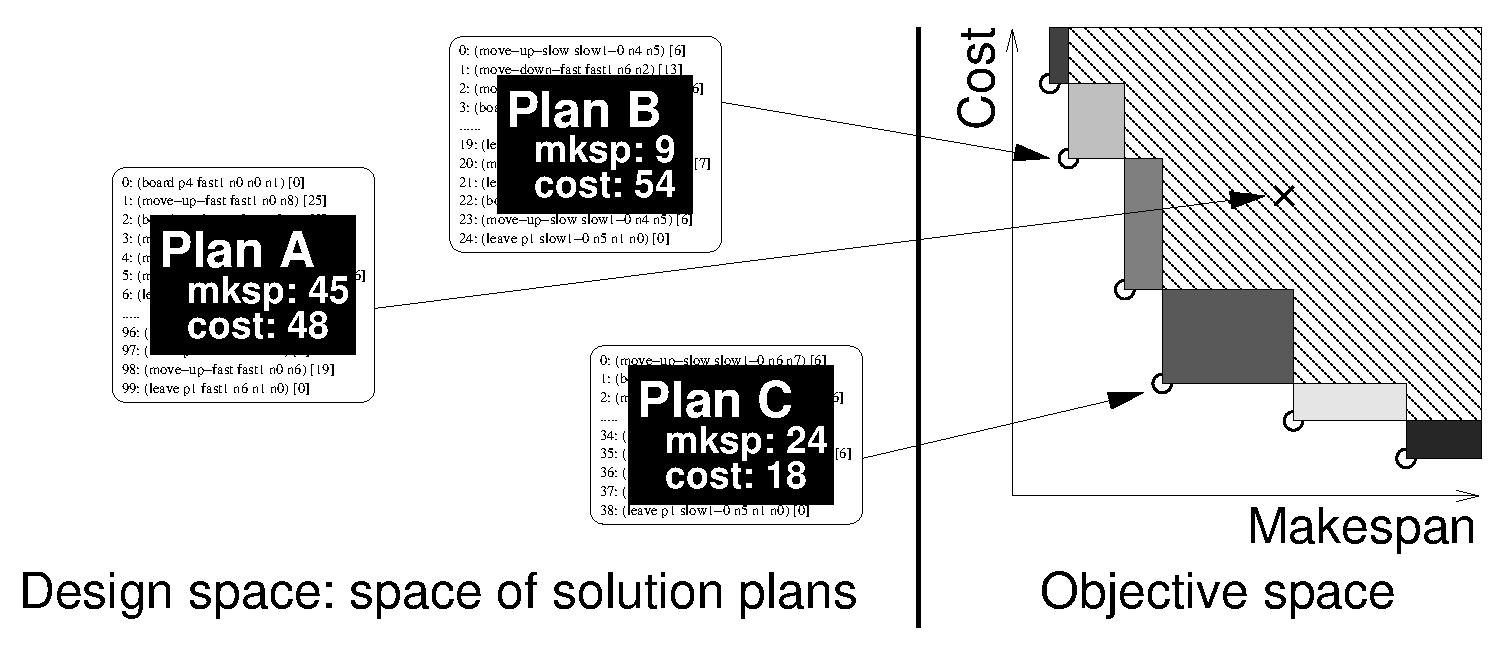
\includegraphics[width=.99\columnwidth]{hypervolumeContributionDAE-V2}}
%\caption{The hypervolume of the set of circle points is the hatched area. The hypervolume contribution of each point is the area of the corresponding small rectangle.}
\caption{Design and objective spaces for a two-objectives planning problem. The hatched+grey area contains all images of possible solutions plans; its area defines the {\em hypervolume} of the set of circles, and the {\em hypervolume contribution} of each point is the grey area of the corresponding small rectangle (see Section \ref{sec:pareto}). Circles are Pareto-optimal (non-dominated) solutions, aka the {\em Pareto front} of the problem at hand.}
\label{fig:hypervolume}
\end{figure}


Sometimes, the user/decision maker might have a very precise idea of the relative losses induced by the degradation of one of the objectives with respect to the improvement of another. It is then possible to turn the multiobjective optimization problem into a single-objective optimization problem, e.g., by optimizing some weighted sum (or any other monotonous function) of the objectives, in the so-called {\em aggregation method}. Any optimizer can then be used to solve the aggregated problem. However, this approach requires some a priori knowledge of the trade-off between the objectives, and/or numerous runs of the optimizer on different aggregations of the objectives. Furthermore, linear aggregation (the weighted sum case) is not able to identify the complete Pareto front in case it is not convex. 

On the other hand, Pareto-based multiobjective algorithms propose a different approach to multiobjective optimization: their goal is to directly identify (a good approximation of) the complete Pareto front, and the corresponding set of solutions of the design space approximating the Pareto set. This latter set can then be proposed to the decision maker so that she/he can make an informed decision when choosing a solution. 
Efficient Pareto-based multiobjective algorithms have been designed using ideas from Evolutionary Algorithms, that can easily be turned into Multiobjective Evolutionary Algorithms (MOEAs) by modifying their selection process to account for Pareto dominance \cite{Deb-book}.

In the domain of AI planning, most works only address single-objective problems, and the very few recent approaches rely on {\em metric-sensitive} planners to optimize metrics built as weighted sums of the objectives (more in Section \ref{sec:multi-planning}). 
This paper introduces \MODAE, the first (to the best of our knowledge) truly Pareto-based Multiobjective AI Planning System. \MODAE\ is a multi-objectivization of \DAE, a domain-independent satisficing planner that has been originally designed for single-objective planning \cite{evoCOP2006,Bibai2010}, and won the IPC-7 temporal deterministic satisficing track at ICAPS 2011. \DAE\ uses an Evolutionary Algorithm (EA) to evolve sequences of partial states for the problem at hand, calling an embedded planner to solve in turn each subproblem of the sequence. If the embedded planner is able to compute metrics along any plan it builds, then \MODAE\ will take care of the global search for the Pareto front, without the need for the embedded planner to be metric-sensitive. After a brief survey of Multiobjective Evolutionary Algorithms (MOEAs, Section \ref{sec:pareto}), Section \ref{sec:pareto-multi-planning} details \DAE\ and \MODAE.

% \DAE\ can embed any existing planner, and has been successful with both the optimal planner CPT \cite{vidal:aaai04} and the lookahead heuristic-based satisficing planner \YAHSP\ \cite{Vidal2004}. \DAE\ uses an Evolutionary Algorithm (EA) to evolve sequences of partial states for the problem at hand, calling the embedded planner to solve in turn each of the subproblems. However, any single-objective EA can easily be turned into a multiobjective EA (MOEA): only the selection part of the EA needs to be modified, using the notion of Pareto-dominance when comparing solutions rather than simply comparing their fitness values \cite{Deb-book} (more in Section \ref{sec:pareto}). Hence turning \DAE\ into \MODAE\ was rather straightforward, and will be detailed in Section \ref{sec:pareto-multi-planning}. 

% \begin{figure}
%  \includegraphics[width=4.5cm]{Figures/figuresOlga/dominanceCSDL.png}
% \caption{Dominance}
% \end{figure}

% The rest of the paper is organized as follows. AI Planning and the recent metric-based multiobjective approaches are introduced in Section \ref{sec:multi-planning}. Section \ref{sec:pareto} presents the bases of Multiobjective Evolutionary Algorithms, including the hypervolume performance indicator and $IBEA_{hyp}$, the base algorithm that has been chosen to multi-objectivize \DAE. Section \ref{sec:DAE} details \DAE\ and its multiobjective variant, \MODAE. 
However, whereas there exist many single-objective planning benchmarks, thanks to the IPC competitions, none has been proposed yet for multiobjective planning. Both a specific tunable artificial benchmark, and a general method to turn some well-known IPC benchmarks into multiobjective domains are presented in Section \ref{sec:benchmarks}.  \MODAEYAHSP, an instantiation of \MODAE\ using YAHSP \cite{Vidal2004} as embedded planner, is validated on these instances, and compared to the results of 
the metric-based approach using the metric-sensitive planner LPG \cite{gerevini2008}, following \cite{LPG-PlanSIG2012}. Finally, Section \ref{sec:conclusion} discusses these results and sketches the directions of further researches.

\section{Multiobjective AI Planning}
\label{sec:multi-planning}

Temporal planning and numerical state variables have been formalized in PDDL2.1 \cite{PDDL2}, as well as metric functions that allow to optimize an aggregation of some criteria based on time and numerical variables. This language has been extended  in PDDL3 \cite{gerevini2006preferences} in order to express preferences and soft constraints, which de facto increase the expressivity and complexity of the metric function to be optimized. However, even though optimizing such functions is a standard way to tackle multiobjective optimization problems, its extension to Pareto-based multiobjective optimization is not straightforward and nothing had been proposed in AI Planning for that purpose until very recently. Indeed, all the literature about multi-criteria/objective planning, such as the works on the planners GRT \cite{Refanidis03}, SAPA \cite{Do2003sapa} or LPG \cite{gerevini2008}, are concerned by optimizing an aggregation of the objectives.

The concept of metric-sensitive planners has been recently defined in \cite{LPG-STAIRS2012}, in order to identify planners able to give diverse solutions when faced with --possibly small-- variations of the metric function. With such a planner, the Pareto front can be approximated by adequately weighting an aggregation of the objectives and running the planner several times within some time limits. An example of such a metric function is $\alpha\times\mathtt{makespan}+(1-\alpha)\times\mathtt{cost}$, where alpha is sampled in $[0,1]$.  Among several candidates: LPRGP \cite{LPRGP}, POPF \cite{POPF}, and LPG, the latter exhibited by far the best performance in terms of metric sensitivity and generated Pareto front quality, and was used in further experiments \cite{LPG-PlanSIG2012}. For this reason, this approach, named here \MOLPG, will also be used as a baseline for the validation of our approach (Section \ref{sec:experiments}). To overcome the metric-insensitivity 
limitation of other planners, \cite{LPG-STAIRS2012} suggest to add artificial bounds on numerical variables, which gave comparable results with the other 
planners in comparison with \MOLPG. However, this requires significantly more engineering, as defining the bounds requires an in-depth analysis of the planning problem, while defining the objective weights is straightforward.


\section{Multiobjective Evolutionary Algorithms}
\label{sec:pareto}

Evolutionary Algorithms (EAs) \cite{EibenSmith2003} are heuristic stochastic search algorithms that crudely mimic natural evolution. A population of individuals (a set of potential solutions in the search space) evolves according to two main drives: reproduction through blind variations (random moves in the search space) and natural selection, aka ``survival of the fittest''. Blind variations depend on the search space, and are usually classified into crossover operators, that involve two or more parent individuals to create one offspring, and mutation operators, that modify a single parent to create one offspring. Selection is applied to choose which parents will reproduce, and also which from the parents plus offspring will survive to the next generation. It can be deterministic or stochastic, but has to be biased toward the fittest individuals. 

In the case of single-objective optimization of some objective function $\cal F$ (e.g., to be minimized), the fitness of an individual $x$ simply is the value ${\cal F}(x)$. In the case of multiobjective optimization, however, Pareto-dominance is not a total order, and hence cannot be used as sole selection criterion. Several Pareto-based Multiobjective Evolutionary Algorithms (MOEAs) have thus been proposed, that use some diversity measure as a secondary criterion when Pareto-dominance cannot distinguish between individuals. 

Several indicators have been proposed for comparing the results of different multiobjective optimization algorithms, i.e., that compare sets of solutions. The most popular is the {\em hypervolume indicator}, because it is the only one that has been proved to be consistent with the Pareto-dominance relation. But indicators can also be used to build a fitness function for some MOEAs: the fitness of an individual (compared to the other individuals in the population) is its contribution to the indicator of the population, i.e., the difference between the indicator of the whole population and that of the population without it. Such MOEAs are called {\em Indicator Based Evolutionary Algorithms} (IBEA) \cite{Zitzler2004} -- and \IBEAH, that will be used throughout this paper, is the one using the hypervolume indicator.


\section{Divide-and-Evolve}
\label{sec:DAE}

\subsection{Single-Objective Divide-and-Evolve}
This section introduces the main characteristics of the satisficing planner \DAE, referring to \cite{Bibai2010} for  comprehensive presentation.
\DAE\ aims at finding a state decomposition of a planning problem $P=\langle A, O, I, G\rangle$, and turns such decomposition problem into an optimization problem: search for a sequence $(s_i)_{i\in [0,n+1]}$, with $s_0=I$ and $s_{n+1}=G$, such that the plan $\sigma$ obtained by compressing subplans $\sigma_i$ found by some embedded planner as solutions of $P_i=\langle A, O, \hat{s}_i, s_{i+1}\rangle_{i\in[0, n]}$ has the best possible quality (with $\hat{s_i}$ denoting the final state reached by applying $\sigma_{i-1}$ from $\hat{s}_{i-1}$). In order to limit the combinatorial explosion of state size, each state $(s_i)_{i\in [1,n]}$ is sought as a partial state, and \DAE\ relies on the admissible heuristic function $h^1$ \cite{HaslumGeffner-AIPS-2000} to restrict the atoms used to describe the states: only the ones that are possibly true according to $h^1$ are considered. Furthermore, mutually exclusive atoms, which can be computed at low cost, are also forbidden in intermediate states $s_i$. These two 
rules are 
strictly imposed during the 
random initialization phase, and progressively relaxed during the search phase. 

Due to the weak structure of the search space (variable-length sequences of variable-length lists of atoms), Evolutionary Algorithms (EAs) have been chosen as the method of choice: EAs are hyper-heuristics that are flexible enough to explore such spaces, as long as they are provided with some stochastic {\em variation operators} (aka {\em move operators} in the heuristic search community) -- and of course some objective function to optimize. 

{\em Variation operators} in \DAE\ are (i) a crossover operator, a straightforward adaptation of the standard one-point crossover to variable-length sequences; and (ii) different mutation operators, that modify the sequence at hand either at the level of the partial states, or at the level of the atoms of one particular state, randomly adding or removing one item, while nevertheless satisfying $h^1$ and mutex-free restrictions.

The objective (aka {\em fitness}) function is obtained by running the embedded planner on the different subproblems, and eventually compressing the corresponding solution plans, if all subproblems were solved. If one subproblem is not solved, the sequence is said to be infeasible, and the fitness is heavily penalized.
\DAE\ can embed any existing planner, and has to-date been successful with both the optimal planner CPT \cite{vidal:aaai04} and the lookahead heuristic-based satisficing planner \YAHSP\ \cite{Vidal2004}. The latter has been demonstrated to outperform the former when used within \DAE\ \cite{bibai-EvoCOP2010}, so only \DAEYAHSP\ has been considered in this work.

\subsection{Multiobjective Divide-and-Evolve}
\label{sec:pareto-multi-planning}

Two modifications of \DAEYAHSP\ are needed to turn it into a MOEA: (i) use some multiobjective selection (Section \ref{sec:pareto}) in lieu of the single-objective tournament selection that is used in the single-objective context; (ii) use the embedded planner to compute the values of both objectives (e.g., makespan and cost). The former modification is straightforward, and several alternatives have been experimented within \cite{nous-emo2013}. The conclusion is that $IBEA_H$ \cite{Zitzler2004} (see Section \ref{sec:pareto}) performs best on instances \MULTIZENO\ (see Section \ref{sec:benchmarks}) -- and only this one will be mentioned in the following.

As explained above, the computation of the fitness is done by \YAHSP\ -- and \YAHSP, like all known planners to-date, is a single-objective planner. It is nevertheless possible, since PDDL 2.1, to specify other metrics that are to be computed throughout the execution of the final plan. For the metric-sensitive planners, this metric is directly used to bias the search, while some other planners, like \YAHSP, simply compute it along the solution plan without interfering with the search. However, because \YAHSP\ is both a temporal planner and a cost planner, two strategies are possible for \YAHSP\ within \MODAE: it can be asked to optimize only the makespan (resp. the cost), and to simply compute the cost (resp. the makespan) when executing the solution plan. 
% The corresponding strategies will be referred to as \YAHSP$_{makespan}$ and \YAHSP$_{cost}$. 

In \MODAEYAHSP, the choice between both strategies is governed by user-defined weights.
% , named respectively \WMAKESPAN\ and \WCOST. 
For each individual, the actual strategy is randomly chosen according to those weights, and applied to all subproblems of the individual. Another important feature of \YAHSP\ for the computation of the objectives of \MODAEYAHSP\ is its stochasticity: \YAHSP\ can explore the plan space stochastically, and different runs on the same instance will give different answers with different random seeds. The effect of the \YAHSP\ strategy % as well as \YAHSP\ 
can be observed on Figure \ref{fig:strategies}, that represent the different objective values of the same individual obtained within \MODAEYAHSP\ when \YAHSP\ uses either the makespan strategy, or the cost strategy, or strategies that are independently randomly chosen for each subproblem: the bias is clear when a unique strategy is chosen for the \MULTIZENO9 instance, and the corresponding part of the objective space is sampled, while the hybrid strategy spreads the values in-between these two clouds of points. Note that on some other instances (\OPENSTACKS, \FLOORTILE, see Section \ref{sec:benchmarks}), the three strategies are absolutely indistinguishable (not shown here).

Some preliminary experiments were also conducted in order to try to take advantage of the stochastic nature of \YAHSP\ evaluations, running \YAHSP\ several times for each individual and keeping the best plan. But surprisingly, even without considering the additional CPU cost, such approach proved detrimental on the quality of the Pareto approximation: such observation had also been made when trying to hybridize EAs with local search methods (iterated \YAHSP\ can indeed be viewed as some sort of local search) - the local search should not try to improve the solutions too early.

Final note regarding the evaluation: the strategy weights, like all parameters of \MODAEYAHSP, have been tuned using ParamILS (see Section \ref{sec:conditions}), and it turned out that the optimal values for \MODAEYAHSP\ have always been equal weights: something that was to be expected, as no objective should be preferred to the other. 

\section{Benchmark Domains and Instances}
\label{sec:benchmarks}
Two approaches were used to design multiobjective benchmark problems: first, using a highly simplified version of the well-known IPC domain \ZENOTRAVEL, a simple and easy to tune domain was built, and the exact Pareto front can be easily identified for all its instances. The other approach is based on modifying IPC-7 problems.


\subsection{\MULTIZENO\ Instances}
\label{ZenoBenchmarks}
\begin{tiny}
\begin{figure}[tb]

\begin{tabular}{cc}
 \includegraphics[height=0.6\columnwidth,angle=270]{./generiqueMiniMulti.ps} 
& 
\begin{tiny}
\begin{tabular}[t]{|m{.25cm}||m{.15cm}|m{.15cm}|m{.15cm}|}
\hline
Dur. & A & B & C \\
\hline 
1 & 2 & 2 & 2\\
2 & 4 & 4 & {\bf 3}\\
3 & 6 & 6 & {\bf 4}\\
4 & 3 & 3 & {\bf 1}\\
5 & 5 & 5 & {\bf 2}\\
6 & 3 & 3 & {\bf 1}\\
7 & 2 & 2 & 2\\
8 & 4 & 4 & {\bf 3}\\
9 & 6 & 6 & {\bf 4}\\
\hline \hline
Cost & & & \\
\hline
1 &  30 & 30 & 30\\
2 & 20 & {\bf 11} &{\bf 29}\\
3 & 10 & 10 & 10 \\
\hline
\end{tabular}
\end{tiny}
\end{tabular}
\caption{Schematic view, and 3 instances, of \MULTIZENO\ benchmark. Flight durations are attached to the possible routes (white circles), costs/risks are attached to landing in the central cities (grey circles). Three sets of values are given on the right, corresponding to Pareto fronts of Figure \ref{fig:allParetoFronts}. }
% \vskip -0.2cm
\label{fig:instance}
\end{figure}
\end{tiny}


\begin{figure}[tb]
\hskip -0.5cm
\begin{tabular}{cccc}
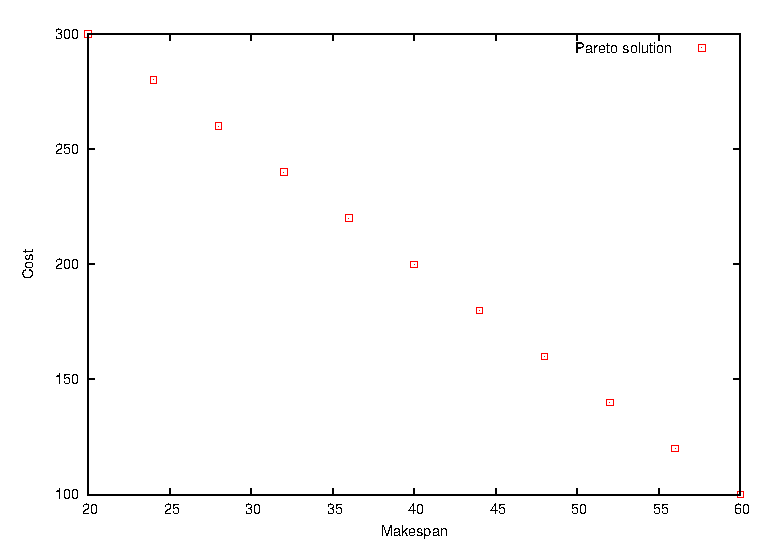
\includegraphics[width=0.32\columnwidth]{../plot_archive/zeno6e10.eps} &
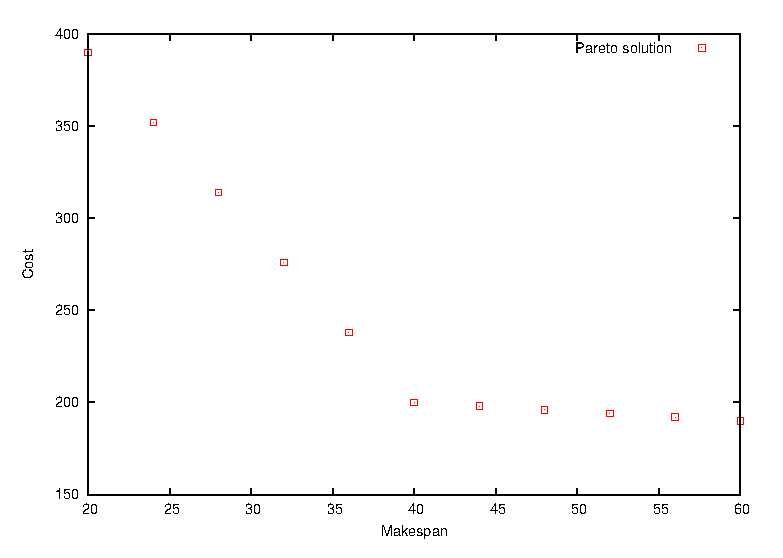
\includegraphics[width=0.32\columnwidth]{../plot_archive/zeno6di.eps} &
% 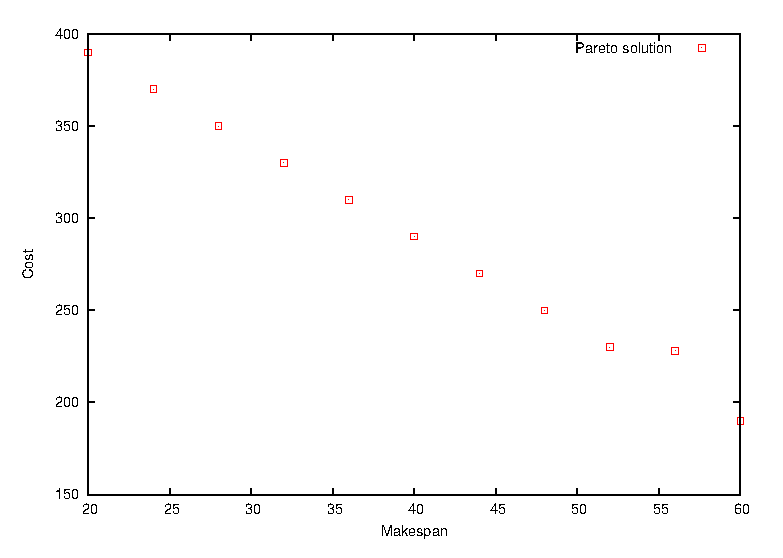
\includegraphics[width=0.24\textwidth]{../plot_archive/zeno6ds.eps} &
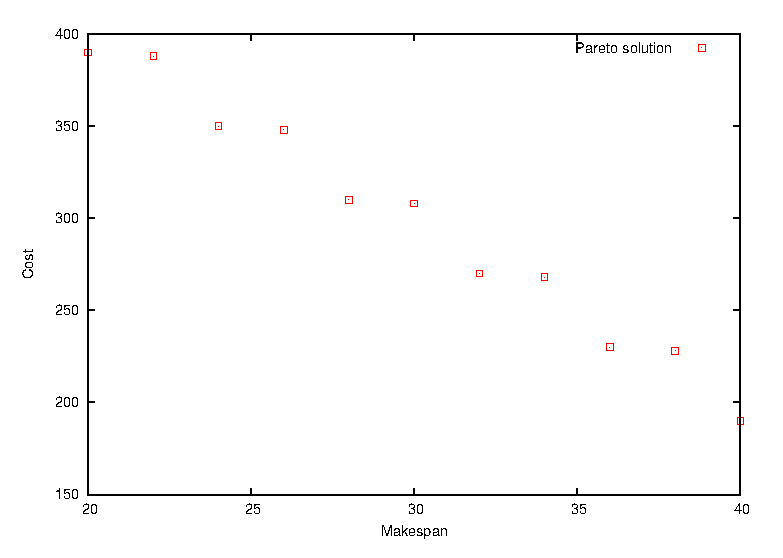
\includegraphics[width=0.32\columnwidth]{../plot_archive/zeno6sc.eps}\\
A - Linear & B - Convex & C - Concave % & More concave 
\end{tabular}
\caption{Pareto Fronts for the instances from Figure \ref{fig:instance}.}
\label{fig:allParetoFronts}
\end{figure}

The \MULTIZENO\ problem domain involves cities, passengers, and planes. One plane can carry at most one passenger from one city to another (action {\tt fly}), following an existing link of Figure \ref{fig:instance}, with corresponding flight durations (see Table). Costs are landing taxes for each of the middle cities. All instances in this work have 2 planes, all passengers are initially in {\tt city 0}, and must reach {\tt city 4}. The simplest non-trivial instance \MULTIZENO3 has 3 passengers. In its default configuration (column A in Table), the makespan-optimal solution has a total makespan of 8, as the reader will easily find out. But all flights have to land in {\tt city 1}, resulting in a cost of 120. The alternative route through  {\tt city 2} (resp. {\tt city 3}) has a makespan of 16 (resp. 24), and a cost of 80 (resp. 40). By increasing the number of passengers, and modifying the flight durations and landing costs, different trade-offs are made possible. Figure \ref{fig:allParetoFronts} displays 
the 3 exact Pareto fronts (in the makespan $\times$ cost space) corresponding to the durations and costs of the table in Figure \ref{fig:instance}, for a total of 6 passengers (aka \MULTIZENO6). 
Note that the second objective could also be considered as a {\em risk} \cite{nous-emo2013}, and the objective is then to minimize the maximum risk encountered during the execution of the plan. This variant of \MULTIZENO\ domain will not be considered here.

\subsection{Multi-Objectivization of IPC Problems}
\label{IPCbenchmarks}
Two satisficing tracks were open at IPC-7: sequential satisficing, i.e., sequential STRIPS planning in which actions have a cost and where the total cost is to be minimized, and temporal satisficing, where actions have a duration and can be run in parallel and where the total makespan is to be minimized\footnote{\url{www.plg.inf.uc3m.es/ipc2011-deterministic}}.
Three possible ways of generating multiobjective instances have been considered. When the domains appeared in both tracks, with the same instances, and when the cost increases as the makespan decreases, a simple merge of both instances is enough. This was the case for domain \ELEVATORS.

% \begin{figure}
% \begin{tiny}
% \begin{verbatim}
% (:action move-up-slow
%    :parameters (?lift - slow-elevator ?f1 - count ?f2 - count)
%    :duration (= ?duration (travel-slow-temp ?f1 ?f2))
%    :precondition (and (lift-at ?lift ?f1) 
%                       (above ?f1 ?f2 )
%                       (reachable-floor ?lift ?f2) )
%    :effect (and (lift-at ?lift ?f2) 
%                 (not (lift-at ?lift ?f1)) 
%                 (increase (total-cost) (travel-slow-cost ?f1 ?f2))))
% \end{verbatim}
% \end{tiny}
% \caption{Typical action of multiobjective {\tt \ELEVATORS}.}
% \label{fig:elevator}
% \end{figure}


For some domains, the cost values of the cost instance did not ensure that both objectives would be antagonist. This is the case for \CREWPLANNING, \FLOORTILE, and \PARCPRINTER. For these instances we arbitrarily set the cost values to a maximum cost minus the value of the duration. \FLOORTILE\ will be the typical domain from this category considered here.
% \begin{figure}
% \begin{tiny}
% \begin{verbatim}
% (:durative-action change_filter
%   :parameters (?fs - FilterState ?c - CrewMember ?d - Day)
%   :duration (= ?duration 60)
%   :condition (and (at start (available ?c))
%                   (over all (currentday ?c ?d)))
%   :effect (and (at start (not (available ?c)))
%                (at end (available ?c))
%                (at end (changed ?fs ?d))
%                (increase (total-cost) (- 10000 60))))
% \end{verbatim}
% \end{tiny}
% \caption{Cost setting in multiobjective {\tt \CREWPLANNING}.}
% \label{fig:crewplanning}
% \end{figure}
Finally, for the \OPENSTACKS\ domain, the cost version has a single costly action, that penalizes the use of a new stack: such scheme is very general in scheduling applications with resources (with more resources, things get done faster, but cost more). For this domain, this cost action was simply added to the temporal domain.

% \begin{figure}
% \begin{tiny}
% \begin{verbatim}
% (:action open-new-stack
%   :duration (= ?duration 1)
%   :parameters (?open ?new-open - count)
%   :precondition (and (stacks-avail ?open)
%                      (next-count ?open ?new-open))
%   :effect (and (not (stacks-avail ?open))
%                (stacks-avail ?new-open) 
%                (increase (total-cost) 1)))
% \end{verbatim}
% \end{tiny}
% \caption{Added cost action of multiobjective {\tt \OPENSTACKS}.}
% \label{fig:openstack}
% \end{figure}


\section{Experiments}
\label{sec:experiments}

The goal of following experiments is to assess the efficiency of \MODAEYAHSP, and its robustness with respect to some variety of planning domains and the size of the instances. The instances presented in Section \ref{sec:benchmarks} will be used in turn, and the performances of \MODAEYAHSP\ will also be assessed against the baseline \MOLPG, the approach proposed in \cite{LPG-PlanSIG2012} (see Section \ref{sec:multi-planning}) which will also be evaluated. The experimental conditions will first be detailed.


\subsection{Parameter Tuning -- Experimental Conditions}
\label{sec:conditions}

\DAEYAHSP, and even more so, \MODAEYAHSP, have a number of free parameters that need to be tuned in order to obtain the best possible results. It is well-known that parameter tuning can make a complete difference between failure and success for the same algorithm on the same problem. In this work, all user-defined parameters have been tuned using the  framework \PARAMILS\
% \footnote{\url{http://www.cs.ubc.ca/labs/beta/Projects/ParamILS/}}~
\cite{ParamILS-JAIR}, that handles any parameterized algorithm whose parameters can be discretized, and uses some Iterated Local Search (ILS) to explore the space of parameter configurations.
Furthermore, because the goal of this work is to demonstrate the efficiency of \MODAE\ to robustly find a good approximation of the Pareto front of multiobjective AI Planning problems, those parameters were tuned anew for one instance of moderate complexity in each domain (see Section \ref{IPCbenchmarks}), and the resulting parameter set was used for all instances of the same domain. This represents a trade-off between CPU cost and performance: there is little hope to ever find some universal parameters for \DAE, that would allow \DAE\ to obtain its best quality performance on all possible instances; on the other hand, such best quality can obviously be obtained by optimizing the parameters anew for each new instance, but at the price of a huge CPU cost. Within \MOLPG, LPG was ran in local-search mode, and given the same overall CPU time for its multiple restarts.

% The extreme points of all Pareto fronts correspond to minimizing one objective without taking care of the other one (except in case of ties on the first objective). Exact extreme points can hence be obtained by running any exact single-objective planner on one of the objectives. When possible, we ran both CPT and Fast Downward Stone Soup-1\footnote{Winner of the Sequential Optimization Track of IPC-7} \cite{FD:IPC2011} to obtain the plans with respectively the minimal makespan and the minimal cost on the same instances, thus obtaining lower bounds for the objective values.

The main goal of the experiments presented here is to assess the ability of \MODAEYAHSP\ to find good quality approximations of the Pareto front. Hence the performances of the different algorithms will be reported w.r.t. the quality of the identified Pareto front after an arbitrary CPU time of 30mn (long enough to allow the algorithms to reach some steady population, as confirmed by preliminary runs). All runs were ran on one core of the same 24-cores server with Xeon X5650@2.67GHz processors, running Ubuntu 10.04 Lucid).
\DAE\ was implement within the \PARADISEO\ framework \cite{paradiseo}. For all experiments, 11 independent runs were performed. All the performance assessment procedures, including the hypervolume calculations, have been achieved using the PISA performance assessment tool suite \cite{Bleuler2003}. % \footnote{\url{http://www.tik.ee.ethz.ch/pisa/}}. 


\subsection{Results on \MULTIZENO\ Instances}
\label{sec:resultsZENO}
Experiments have been conducted on the 3, 6 and 9 passengers versions of \MULTIZENO\ (Section \ref{ZenoBenchmarks}), with the Linear configuration (Figure \ref{fig:allParetoFronts}-a). The \MULTIZENO3 instance proved to be too easy, and both \MODAEYAHSP\ and \MOLPG\ could rapidly find the complete Pareto front. For \MULTIZENO6, the situation is drastically different for \MOLPG, that is only able to find a few points far away from the Pareto front (see Figure \ref{fig:zeno6-lpg-dae}). On the other hand, \MODAEYAHSP\ perfectly identifies the complete Pareto front in all runs for the Linear and Concave cases, while 2 runs out of 11 miss one point each. Finally, when tackling \MULTIZENO9 (and while \MOLPG\ fails to find a single feasible plan), \MODAEYAHSP\ is able to approach the true Pareto front rather robustly, as witnessed by Figure \ref{fig:zeno9-dae}, that represents the aggregated 11 Pareto fronts of the 11 independent runs.


\begin{figure*}[ht!]
   \subfloat[Importance of \YAHSP\ strategy]{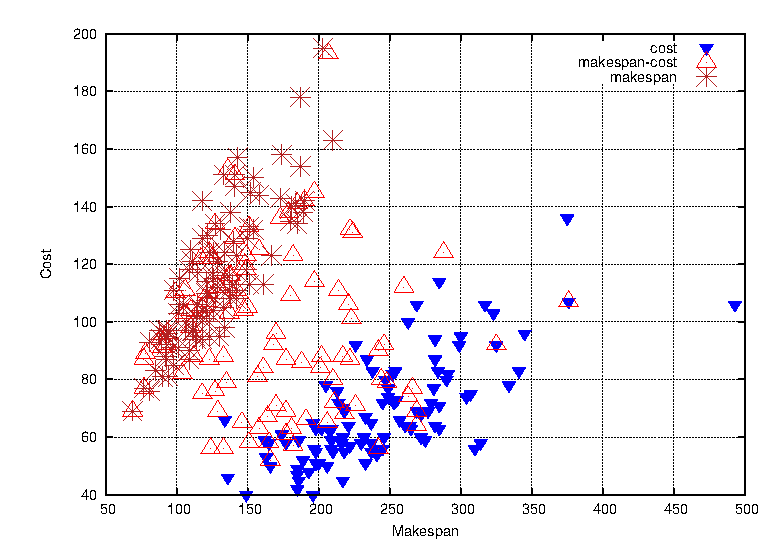
\includegraphics[width=0.32\textwidth,height=3.2cm\label{fig:strategies}] {../plot_archive/zeno9GlobLevelDaeYahsp_Add_dae_pareto1.eps}}
 \subfloat[\MULTIZENO9: exact ($\bullet$) \& approx. ($\blacktriangledown$)\label{fig:zeno9-dae}]{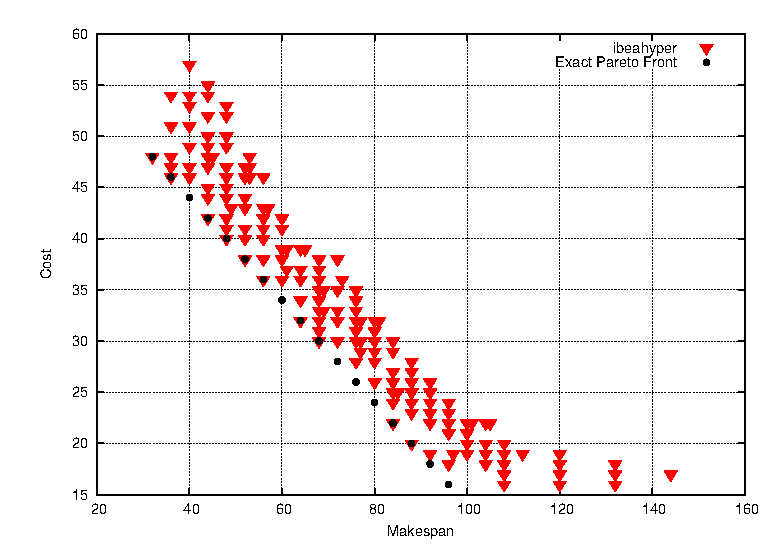
\includegraphics[width=0.32\textwidth,height=3.2cm]{../emo2012/zeno9_Add_ibeahyper-pareto.eps}}
 \subfloat[\MULTIZENO6: \DAE\ ($\blacktriangledown$) vs {\sc LPG} ($\vartriangle$)\label{fig:zeno6-lpg-dae}]{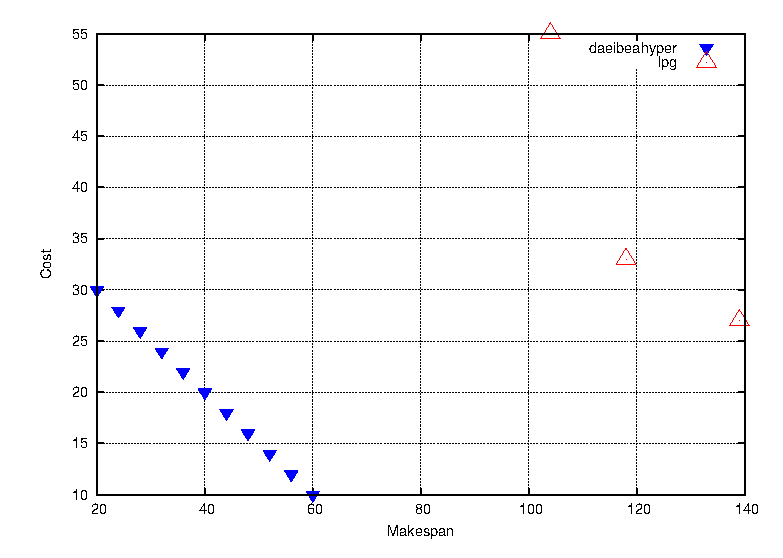
\includegraphics[width=0.32\textwidth,height=3.2cm]{../plot_archive/zeno6eMini_Add_dae_pareto.eps}}
\caption{Experiments on \MULTIZENO\ instances (see text for details).}
\label{fig:paretoFronts}
\end{figure*}



% \begin{figure*}[ht!]
%    \subfloat[\MULTIZENO9]{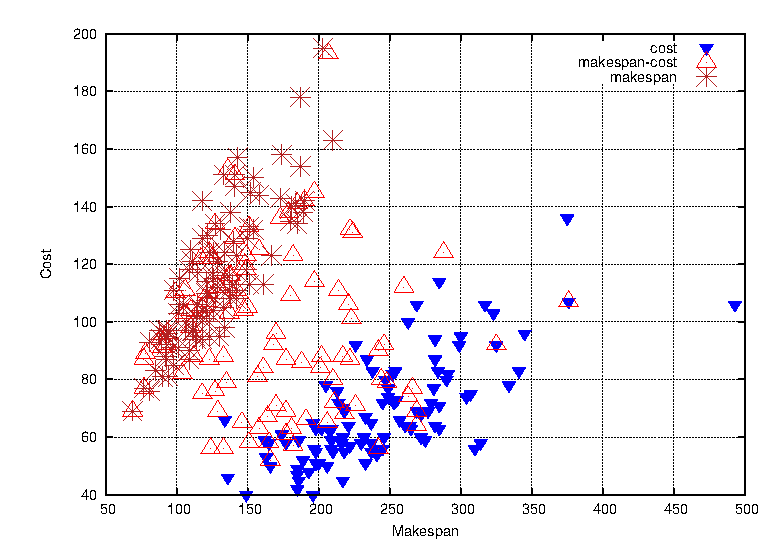
\includegraphics[width=0.32\textwidth,height=3.2cm] {../plot_archive/zeno9GlobLevelDaeYahsp_Add_dae_pareto1.eps}}
%    \subfloat[floortile03]{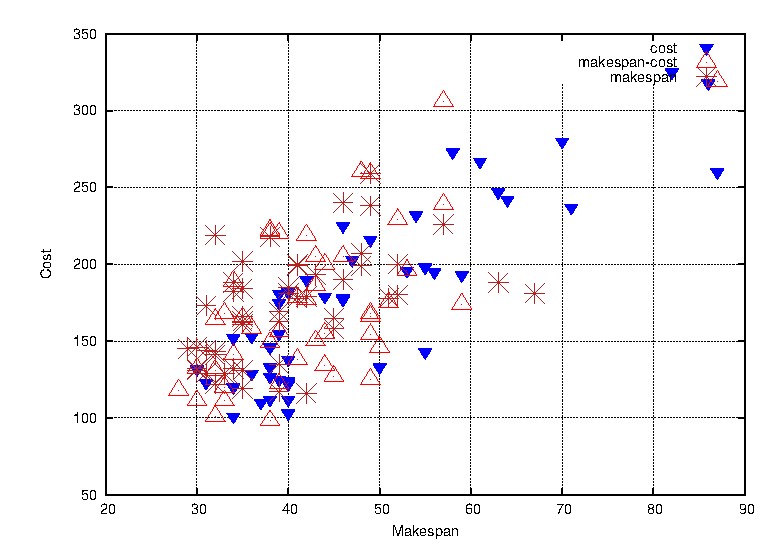
\includegraphics[width=0.32\textwidth,height=3.2cm]{../plot_archive/floortile03DAE_Add__pareto.eps}}
%    \subfloat[openstack15]{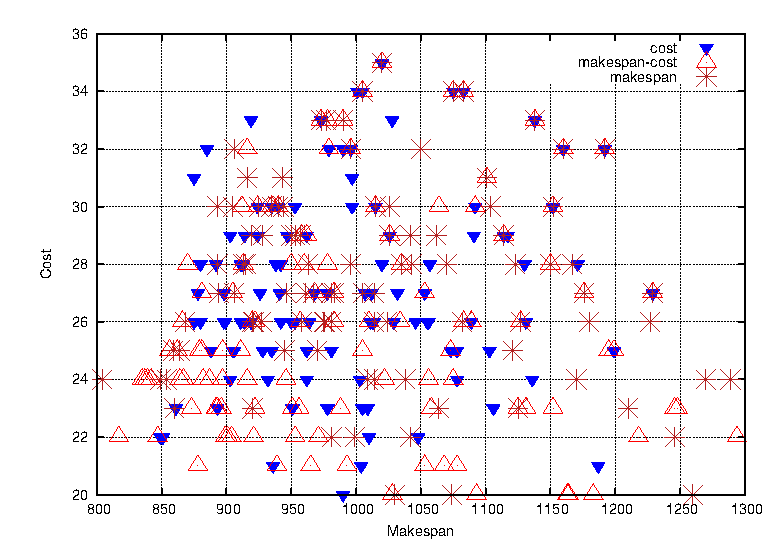
\includegraphics[width=0.32\textwidth,height=3.2cm]{../plot_archive/openstacks15_DAE_Add__pareto.eps}}
% \caption{Objective values of several evaluations of one random individual with different \YAHSP\ strategies: makespan only (*), cost only ($\blacktriangledown$), or one at random for each subgoal ($\vartriangle$)}
% \label{fig:strategies}
% \end{figure*}


\subsection{Results on Modified IPC-7 Instances}
\label{sec:resultsIPC7}

\begin{figure*}[ht!]
  %\subfloat[openstacks05]{\label{openstacks05}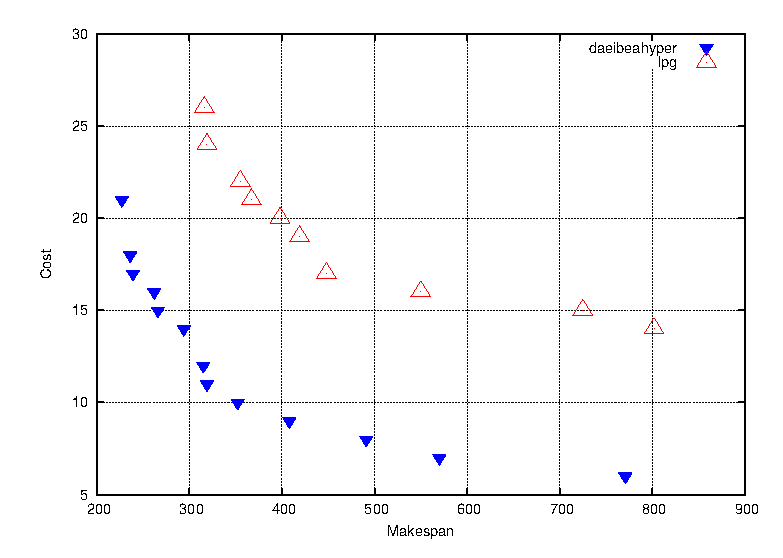
\includegraphics[width=0.32\textwidth,height=3.2cm] {../plot_archive/p05_openstacks_Add_dae_pareto.eps} }
  %\subfloat[openstacks10]{\label{openstacks10}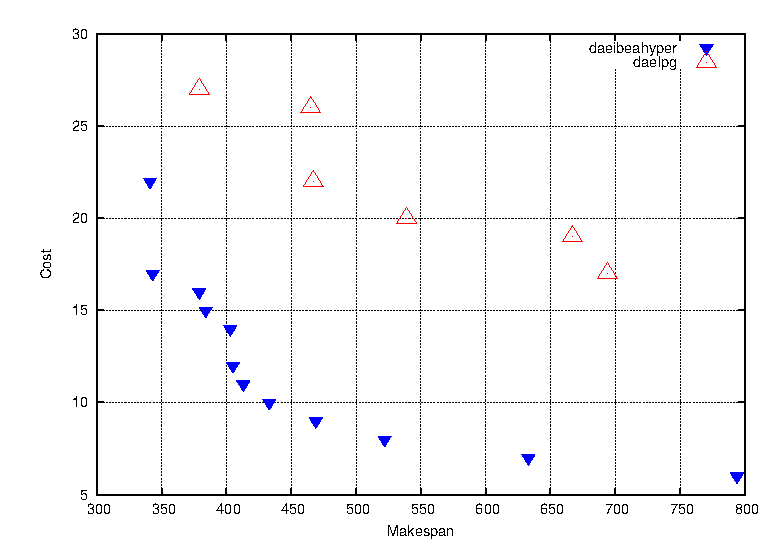
\includegraphics[width=0.32\textwidth,height=3.2cm]{../plot_archive/p10_openstacks_Add_dae_pareto.eps}}
  \subfloat[\ELEVATORS01:\DAE\ ($\blacktriangledown$) vs {\sc LPG} ($\vartriangle$)]{\label{elevators01}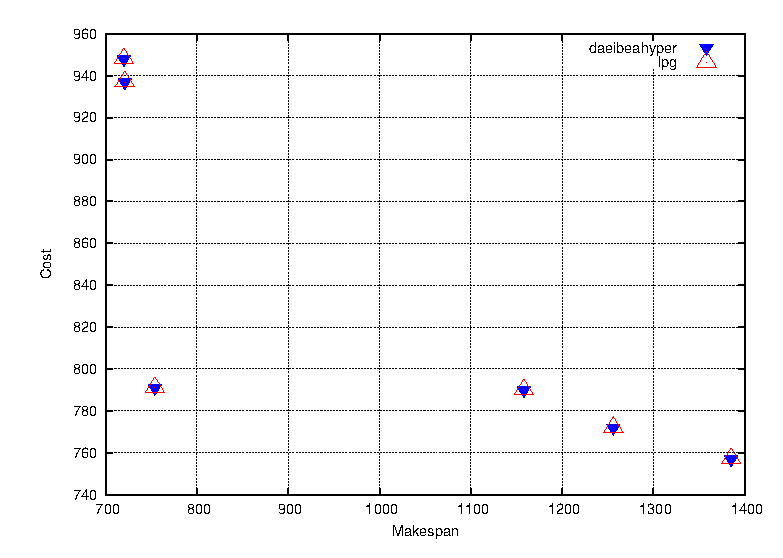
\includegraphics[width=0.32\textwidth,height=3.2cm] {../plot_archive/p01-p04_elevators_Add_dae_pareto.eps} }
  \subfloat[\OPENSTACKS5: \DAE\ ($\blacktriangledown$) vs {\sc LPG} ($\vartriangle$)]{\label{openstacks5}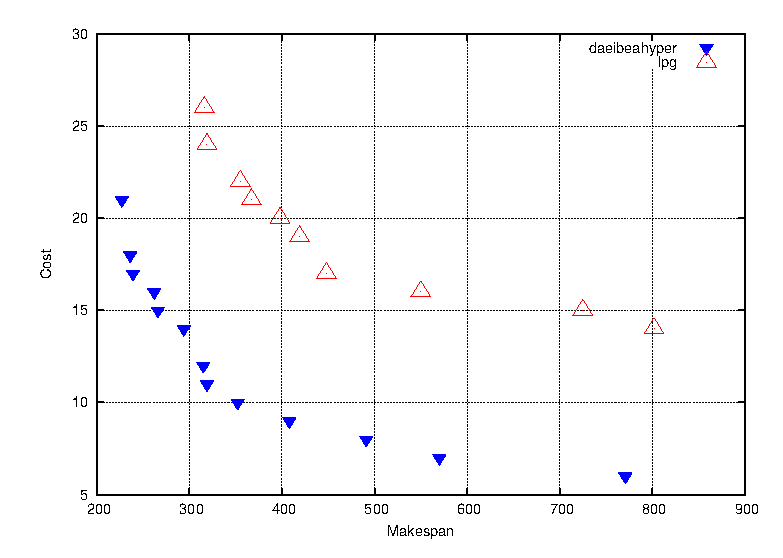
\includegraphics[width=0.32\textwidth,height=3.2cm]{../plot_archive/p05_openstacks_Add_dae_pareto.eps}}
  \subfloat[\FLOORTILE03: \DAE\ ($\blacktriangledown$) vs {\sc LPG} ($\vartriangle$)]{\label{floortile03}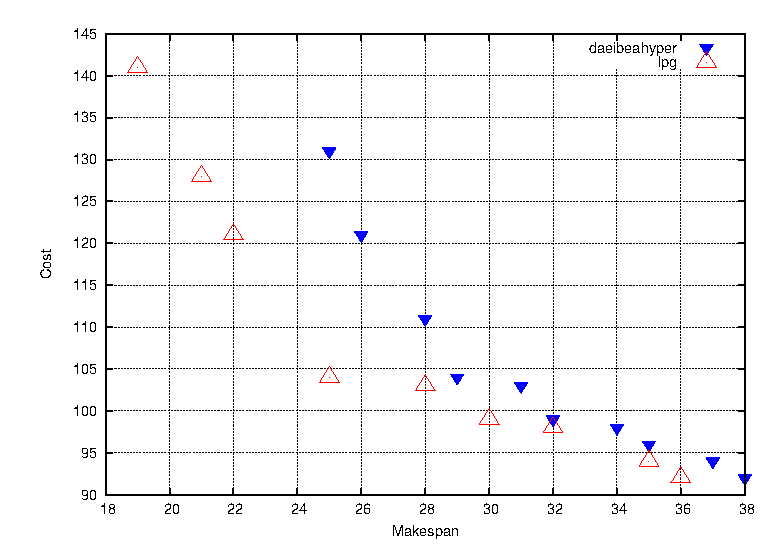
\includegraphics[width=0.32\textwidth,height=3.2cm] {../plot_archive/pfile3_floortile_Add_dae_pareto.eps} }\\
  \subfloat[\ELEVATORS10: \DAE]{\label{elevators10dae}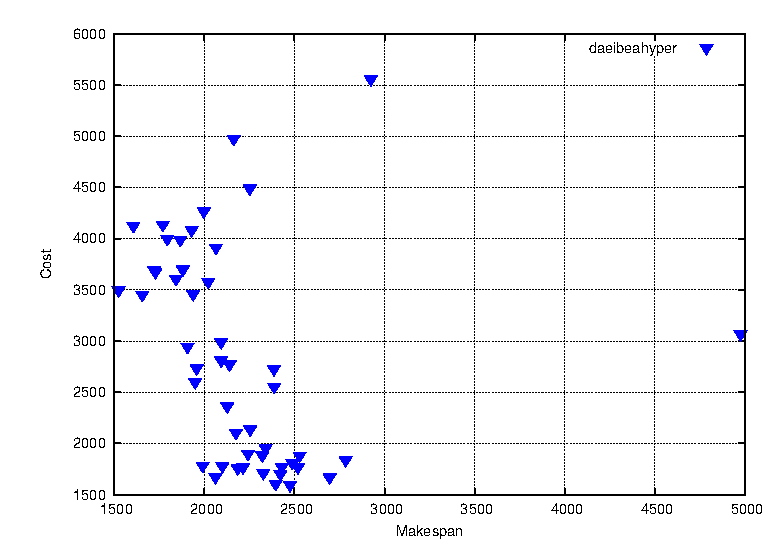
\includegraphics[width=0.32\textwidth,height=3.2cm]{../plot_archive/elevators_p10_Add_ibea_pareto.eps} }
  \subfloat[\OPENSTACKS15: \DAE] {\label{openstacks15dae}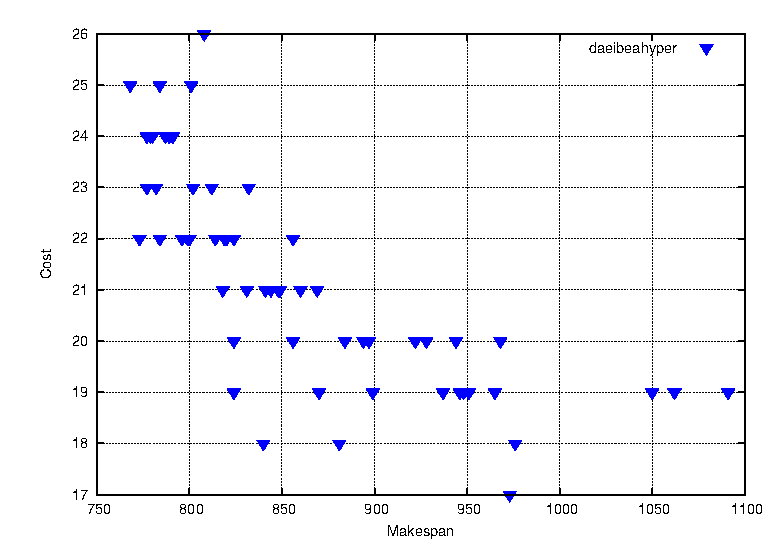
\includegraphics[width=0.32\textwidth,height=3.2cm]{../plot_archive/openstacks_p15_Add_ibea_pareto.eps} }
  \subfloat[\OPENSTACKS15: LPG]{\label{openstacks15lpg}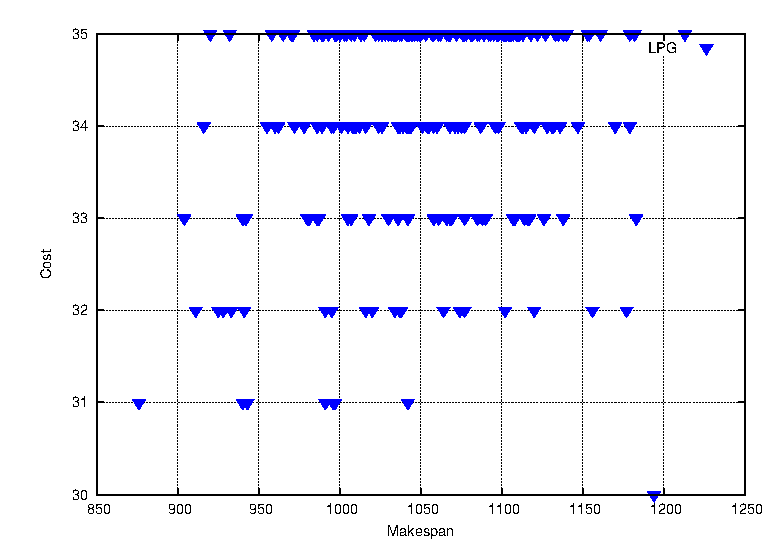
\includegraphics[width=0.32\textwidth,height=3.2cm]{../plot_archive/p15_openstacks_1000_lpg_pareto.eps} }
\caption{Pareto fronts identified by \DAE\ and LPG for multi-objectivized IPC-7 instances (a -- c) and complete solution sets found by \DAE\ (d and e) and by LPG (f).}
\label{fig:ipc7}
\end{figure*}

% The non-antagonistic nature of the objectives is also witnessed by the study of the influence of \YAHSP\ strategy. Figure \ref{fig:strategyElevator} shows that the repartition of the solutions obtained when \YAHSP\ only optimizes the cost or the makespan cover the same area, which is also the area covered by the hybrid strategy governed by equal weights. This is to be compared to Figure \ref{fig:strategyMiniZeno} where the influence of \YAHSP\ is clear.

Figure \ref{fig:ipc7} exhibits some results on multi-objectivized IPC-7 instances (Section \ref{IPCbenchmarks}) for \MODAEYAHSP\ and \MOLPG. Indeed, because the exact Pareto front of these instances is unknown, the only possible assessment of \MODAEYAHSP\ is by comparison to \MOLPG\ results.

For the \ELEVATORS\ domain, instances 1, 5, 10 were experimented. For instance 1 (Figure \ref{elevators01}), \MODAEYAHSP\ and \MOLPG\ find exactly the same Pareto front, but \MOLPG\ is unable to find any solution for instances 5 and above. On the other hand, \MODAEYAHSP\ identifies some Pareto front, as can be seen for instance 10 on Figure \ref{elevators10dae}.

On the \OPENSTACKS\ domain, experiments involved instances 1, 5, 10, 15 and 20. For the small instances (5 -- Figure \ref{openstacks5}, and 1 and 10, not shown), \MODAEYAHSP\ clearly finds a much better Pareto front than \MOLPG. For larger instances (15 and 20, not shown), the situation is even worse for \MOLPG, that only finds very poor solutions (w.r.t. the ones found by \MODAEYAHSP). As an illustration of how both algorithms explore the objective space Figures \ref{openstacks15dae} and \ref{openstacks15lpg} show that the complete solution set computed by \DAE\ (merge of the 11 independent approximations) is nicely distributed along the Pareto front, whereas the solutions of LPG are much more scattered in the design space.

The situation changes for \FLOORTILE\ domain: instances 0, 3 and 4 were used, and here \MOLPG\ outperforms \MODAEYAHSP, as can be seen for instance 3 in Figure \ref{floortile03}.
However, as the instance size increases (instance 4 and above), the gap between LPG and \DAE\ decreases.
% and even more LPG is unable to find solutions in reasonable time for big instances.\mycomments{\bf C'est vrai ?}


\section{Discussion and Conclusion}
\label{sec:conclusion}

Not all planners are metrics-sensitive, in the sense advocated by \cite{LPG-STAIRS2012}: the main contribution of this work has been to demonstrate the ability of the \MODAE\ approach to turn any planner into a multiobjective planner, provided it can reason on either objectives alone (here, the makespan and the cost), as has been done here with \YAHSP. The resulting algorithm is a truly Pareto-based multiobjective planner, that consistently outperforms the metrics-based approach \MOLPG\ on all instances tested here except the small \FLOORTILE\ instances. \MODAEYAHSP\ is able to solve much larger instances, and to find most of the time better approximations of the Pareto front than \MOLPG. 
More work is needed to improve even more the \MODAE\ approach to multiobjective planning. But we strongly believe that the rationale underlying the original \DAE\ is still valid, and that the decomposition-based approach that it implements will push upward the complexity of the problems that we can solve.

The second contribution of this work is the proposition for procedures to build multiobjective benchmark suites for AI Planning. There is no need to advocate the usefulness of large and diverse benchmark suites: in the context of single-objective optimization, advances in research (from the different versions of PDDL to the numerous powerful planners we know of today) have coevolved together with the design of the successive IPC benchmarks. Because multiobjective optimization is mandatory in order to tackle real-world problems, we strongly believe that progress in multiobjective planners requires as well the design of meaningful multiobjective AI Planning benchmarks with gradual difficulties. The \MULTIZENO\ suite detailed here is a first step in this direction: it is a tunable artificial testbed, and was shown to be able to generate interesting Pareto fronts (e.g. convex with a knee as well as non-convex). Furthermore, it has many degrees of freedom that still have not been explored: other combinations of 
durations and makespans, more intermediate cities, with more possible routes between them. 
Another possibility would have been to use the benchmarks designed in \cite{LPG-PlanSIG2012,LPG-STAIRS2012}, but unfortunately the current implementation of \MODAEYAHSP\ relies on YAHSP, which does not handle numerical state variables except for the special case of action costs. However, we believe that multiobjective instances with time and cost objectives are already challenging enough, and could permit the use or extension of many more existing planners which mainly optimize cost or time.
The multi-objectivization of IPC-7 domains is another possible route we have sketched, though more work is still required to transform the single-objective domains into ``interesting'' multiobjective ones, even in the favorable case where both a cost and a temporal version of the same domain already exist. When both objectives are not contradictory enough, setting one as the inverse of the other does the trick, but the Pareto fronts remain close to linear fronts, while more interesting fronts (e.g. non-convex, ``discontinuous'', \ldots) are necessary to test different characteristics of the planners. 
Furthermore, such multiobjective instance can hardly be tackled by state-of-the-art metric-sensitive planners, which are among the only potential competitors as of today: beside the general difficulty of finding the proper weights depending on the objective scales, linear combinations of the objectives can only give in that case one single non-dominated plan, and other aggregations are not guaranteed to lead to points on the Pareto front.
Final word on the modified IPC-7 instances, the failure of LPG on even rather small instances suggests that we should probably have started with easiest instances (e.g., IPC-6?), as the successive competitions have lead to harden even the simplest instances of all IPC domains.

% 
% \textcolor{red}{seeding \DAE\ with LPG solutions ???
% Using more sophisticated measures of performance to compare different algorithms? ???}

%\section{Acknowledgments}

%This work is being partially funded by xxxxxxxxxxxxxxxxxxxxxxxxxxxxxxxxxxxxxxxxx
% the French National Research Agency through the COSINUS program, under the research contract DESCARWIN (ANR-09-COSI-002).

\newpage
%% The file named.bst is a bibliography style file for BibTeX 0.99c
\bibliographystyle{named}
\bibliography{evobib}

\end{document}



\newpage

\onecolumn
% MO-ELEVATORS DOMAIN
\begin{verbatim}
(define (domain elevators-tempo-cost)
  (:requirements :typing :durative-actions :action-costs)
  (:types elevator - object 
          slow-elevator fast-elevator - elevator
          passenger - object
          count - object)

  (:predicates 
    (passenger-at ?person - passenger ?floor - count)
    (boarded ?person - passenger ?lift - elevator)
    (lift-at ?lift - elevator ?floor - count)
    (reachable-floor ?lift - elevator ?floor - count)
    (above ?floor1 - count ?floor2 - count)
    (passengers ?lift - elevator ?n - count)
    (can-hold ?lift - elevator ?n - count)
    (next ?n1 - count ?n2 - count))

  (:functions (total-cost)
    (travel-slow-cost ?f1 - count ?f2 - count)
    (travel-fast-cost ?f1 - count ?f2 - count)
    (travel-slow-temp ?f1 - count ?f2 - count)
    (travel-fast-temp ?f1 - count ?f2 - count))

  (:durative-action move-up-slow
    :parameters (?lift - slow-elevator ?f1 - count ?f2 - count )
    :duration (= ?duration (travel-slow-temp ?f1 ?f2))
    :condition (and (at start (lift-at ?lift ?f1)) (at start (above ?f1 ?f2)) (at start (reachable-floor ?lift ?f2)) )
    :effect (and (at end (lift-at ?lift ?f2)) (at start (not (lift-at ?lift ?f1))) (at end (increase (total-cost) (travel-slow-cost ?f1 ?f2)))))

  (:durative-action move-down-slow
    :parameters (?lift - slow-elevator ?f1 - count ?f2 - count )
    :duration (= ?duration (travel-slow-temp ?f2 ?f1))
    :condition (and (at start (lift-at ?lift ?f1)) (at start (above ?f2 ?f1)) (at start (reachable-floor ?lift ?f2)) )
    :effect (and (at end (lift-at ?lift ?f2)) (at start (not (lift-at ?lift ?f1))) (at end (increase (total-cost) (travel-slow-cost ?f2 ?f1)))))

  (:durative-action move-up-fast
    :parameters (?lift - fast-elevator ?f1 - count ?f2 - count )
    :duration (= ?duration (travel-fast-temp ?f1 ?f2))
    :condition (and (at start (lift-at ?lift ?f1)) (at start (above ?f1 ?f2)) (at start (reachable-floor ?lift ?f2)) )
    :effect (and (at end (lift-at ?lift ?f2)) (at start (not (lift-at ?lift ?f1))) (at end (increase (total-cost) (travel-fast-cost ?f1 ?f2)))))

  (:durative-action move-down-fast
    :parameters (?lift - fast-elevator ?f1 - count ?f2 - count )
    :duration (= ?duration (travel-fast-temp ?f2 ?f1))
    :condition (and (at start (lift-at ?lift ?f1)) (at start (above ?f2 ?f1)) (at start (reachable-floor ?lift ?f2)) )
    :effect (and (at end (lift-at ?lift ?f2)) (at start (not (lift-at ?lift ?f1))) (at end (increase (total-cost) (travel-fast-cost ?f2 ?f1)))))

  (:durative-action board
    :parameters (?p - passenger ?lift - elevator ?f - count ?n1 - count ?n2 - count)
    :duration (= ?duration 1)
    :condition ( and  (over all (lift-at ?lift ?f)) (at start (passenger-at ?p ?f)) (at start (passengers ?lift ?n1)) (at start (next ?n1 ?n2)) (at start (can-hold ?lift ?n2)) )
    :effect (and (at start (not (passenger-at ?p ?f))) (at end (boarded ?p ?lift)) (at start (not (passengers ?lift ?n1))) (at end (passengers ?lift ?n2))))

  (:durative-action leave 
    :parameters (?p - passenger ?lift - elevator ?f - count ?n1 - count ?n2 - count)
    :duration (= ?duration 1)
    :condition ( and  (over all (lift-at ?lift ?f)) (at start (boarded ?p ?lift)) (at start (passengers ?lift ?n1)) (at start (next ?n2 ?n1)) )
    :effect (and (at end (passenger-at ?p ?f)) (at start (not (boarded ?p ?lift))) (at start (not (passengers ?lift ?n1))) (at end (passengers ?lift ?n2))))
  
)
\end{verbatim}

% MO-ELEVATORS p01-p04-temp-cost.pddl PROBLEM
\begin{verbatim}
(define (problem elevators-time-cost-p01-p04)
  (:domain elevators-tempo-cost)
  (:objects 
     n0 n1 n2 n3 n4 n5 n6 n7 n8 n9 n10 n11 n12 n13 n14 n15 n16  - count
     p0 p1 p2 p3 p4 p5 p6 p7 p8 p9 p10 p11 p12 p13 p14 p15 p16 p17 p18 p19 p20 p21 p22 p23 p24 p25  - passenger
     fast0 fast1  - fast-elevator
     slow0-0 slow1-0 - slow-elevator)

  (:init
     (next n0 n1) (next n1 n2) (next n2 n3) (next n3 n4) (next n4 n5) (next n5 n6) (next n6 n7) (next n7 n8) (next n8 n9) (next n9 n10) (next n10 n11) (next n11 n12) (next n12 n13) (next n13 n14) (next n14 n15) (next n15 n16) 

     (above n0 n1) (above n0 n2) (above n0 n3) (above n0 n4) (above n0 n5) (above n0 n6) (above n0 n7) (above n0 n8) (above n0 n9) (above n0 n10) (above n0 n11) (above n0 n12) (above n0 n13) (above n0 n14) (above n0 n15) (above n0 n16) 
     (above n1 n2) (above n1 n3) (above n1 n4) (above n1 n5) (above n1 n6) (above n1 n7) (above n1 n8) (above n1 n9) (above n1 n10) (above n1 n11) (above n1 n12) (above n1 n13) (above n1 n14) (above n1 n15) (above n1 n16) 
     (above n2 n3) (above n2 n4) (above n2 n5) (above n2 n6) (above n2 n7) (above n2 n8) (above n2 n9) (above n2 n10) (above n2 n11) (above n2 n12) (above n2 n13) (above n2 n14) (above n2 n15) (above n2 n16) 
     (above n3 n4) (above n3 n5) (above n3 n6) (above n3 n7) (above n3 n8) (above n3 n9) (above n3 n10) (above n3 n11) (above n3 n12) (above n3 n13) (above n3 n14) (above n3 n15) (above n3 n16) 
     (above n4 n5) (above n4 n6) (above n4 n7) (above n4 n8) (above n4 n9) (above n4 n10) (above n4 n11) (above n4 n12) (above n4 n13) (above n4 n14) (above n4 n15) (above n4 n16) 
     (above n5 n6) (above n5 n7) (above n5 n8) (above n5 n9) (above n5 n10) (above n5 n11) (above n5 n12) (above n5 n13) (above n5 n14) (above n5 n15) (above n5 n16) 
     (above n6 n7) (above n6 n8) (above n6 n9) (above n6 n10) (above n6 n11) (above n6 n12) (above n6 n13) (above n6 n14) (above n6 n15) (above n6 n16) 
     (above n7 n8) (above n7 n9) (above n7 n10) (above n7 n11) (above n7 n12) (above n7 n13) (above n7 n14) (above n7 n15) (above n7 n16) 
     (above n8 n9) (above n8 n10) (above n8 n11) (above n8 n12) (above n8 n13) (above n8 n14) (above n8 n15) (above n8 n16) 
     (above n9 n10) (above n9 n11) (above n9 n12) (above n9 n13) (above n9 n14) (above n9 n15) (above n9 n16) 
     (above n10 n11) (above n10 n12) (above n10 n13) (above n10 n14) (above n10 n15) (above n10 n16) 
     (above n11 n12) (above n11 n13) (above n11 n14) (above n11 n15) (above n11 n16) 
     (above n12 n13) (above n12 n14) (above n12 n15) (above n12 n16) 
     (above n13 n14) (above n13 n15) (above n13 n16) 
     (above n14 n15) (above n14 n16) 
     (above n15 n16) 

     (lift-at fast0 n16)
     (passengers fast0 n0)
     (can-hold fast0 n1) (can-hold fast0 n2) (can-hold fast0 n3) (can-hold fast0 n4) 
     (reachable-floor fast0 n0)(reachable-floor fast0 n4)(reachable-floor fast0 n8)(reachable-floor fast0 n12)(reachable-floor fast0 n16)

     (lift-at fast1 n8)
     (passengers fast1 n0)
     (can-hold fast1 n1) (can-hold fast1 n2) (can-hold fast1 n3) (can-hold fast1 n4) 
     (reachable-floor fast1 n0)(reachable-floor fast1 n4)(reachable-floor fast1 n8)(reachable-floor fast1 n12)(reachable-floor fast1 n16)

     (lift-at slow0-0 n5)
     (passengers slow0-0 n0)
     (can-hold slow0-0 n1) (can-hold slow0-0 n2) (can-hold slow0-0 n3) 
     (reachable-floor slow0-0 n0)(reachable-floor slow0-0 n1)(reachable-floor slow0-0 n2)(reachable-floor slow0-0 n3)(reachable-floor slow0-0 n4)(reachable-floor slow0-0 n5)(reachable-floor slow0-0 n6)(reachable-floor slow0-0 n7)(reachable-floor slow0-0 n8)

     (lift-at slow1-0 n13)
     (passengers slow1-0 n0)
     (can-hold slow1-0 n1) (can-hold slow1-0 n2) (can-hold slow1-0 n3) 
     (reachable-floor slow1-0 n8)(reachable-floor slow1-0 n9)(reachable-floor slow1-0 n10)(reachable-floor slow1-0 n11)(reachable-floor slow1-0 n12)(reachable-floor slow1-0 n13)(reachable-floor slow1-0 n14)(reachable-floor slow1-0 n15)(reachable-floor slow1-0 n16)

     (passenger-at p0 n16)
     (passenger-at p1 n7)
     (passenger-at p2 n0)
     (passenger-at p3 n0)
     (passenger-at p4 n10)
     (passenger-at p5 n15)
     (passenger-at p6 n8)
     (passenger-at p7 n14)
     (passenger-at p8 n4)
     (passenger-at p9 n12)
     (passenger-at p10 n12)
     (passenger-at p11 n4)
     (passenger-at p12 n6)
     (passenger-at p13 n12)
     (passenger-at p14 n2)
     (passenger-at p15 n15)
     (passenger-at p16 n14)
     (passenger-at p17 n2)
     (passenger-at p18 n12)
     (passenger-at p19 n10)
     (passenger-at p20 n7)
     (passenger-at p21 n16)
     (passenger-at p22 n2)
     (passenger-at p23 n16)
     (passenger-at p24 n10)
     (passenger-at p25 n13)

     (= (travel-slow-temp n0 n1) 12) (= (travel-slow-temp n0 n2) 20) (= (travel-slow-temp n0 n3) 28) (= (travel-slow-temp n0 n4) 36) (= (travel-slow-temp n0 n5) 44) (= (travel-slow-temp n0 n6) 52) (= (travel-slow-temp n0 n7) 60) (= (travel-slow-temp n0 n8) 68) (= (travel-slow-temp n1 n2) 12) (= (travel-slow-temp n1 n3) 20) (= (travel-slow-temp n1 n4) 28) (= (travel-slow-temp n1 n5) 36) (= (travel-slow-temp n1 n6) 44) (= (travel-slow-temp n1 n7) 52) (= (travel-slow-temp n1 n8) 60) (= (travel-slow-temp n2 n3) 12) (= (travel-slow-temp n2 n4) 20) (= (travel-slow-temp n2 n5) 28) (= (travel-slow-temp n2 n6) 36) (= (travel-slow-temp n2 n7) 44) (= (travel-slow-temp n2 n8) 52) (= (travel-slow-temp n3 n4) 12) (= (travel-slow-temp n3 n5) 20) (= (travel-slow-temp n3 n6) 28) (= (travel-slow-temp n3 n7) 36) (= (travel-slow-temp n3 n8) 44) (= (travel-slow-temp n4 n5) 12) (= (travel-slow-temp n4 n6) 20) (= (travel-slow-temp n4 n7) 28) (= (travel-slow-temp n4 n8) 36) (= (travel-slow-temp n5 n6) 12) (= (travel-slow-temp n5 n7)
 20) (= (travel-slow-temp n5 n8) 28) (= (travel-slow-temp n6 n7) 12) (= (travel-slow-temp n6 n8) 20) (= (travel-slow-temp n7 n8) 12) 

     (= (travel-slow-temp n8 n9) 12) (= (travel-slow-temp n8 n10) 20) (= (travel-slow-temp n8 n11) 28) (= (travel-slow-temp n8 n12) 36) (= (travel-slow-temp n8 n13) 44) (= (travel-slow-temp n8 n14) 52) (= (travel-slow-temp n8 n15) 60) (= (travel-slow-temp n8 n16) 68) (= (travel-slow-temp n9 n10) 12) (= (travel-slow-temp n9 n11) 20) (= (travel-slow-temp n9 n12) 28) (= (travel-slow-temp n9 n13) 36) (= (travel-slow-temp n9 n14) 44) (= (travel-slow-temp n9 n15) 52) (= (travel-slow-temp n9 n16) 60) (= (travel-slow-temp n10 n11) 12) (= (travel-slow-temp n10 n12) 20) (= (travel-slow-temp n10 n13) 28) (= (travel-slow-temp n10 n14) 36) (= (travel-slow-temp n10 n15) 44) (= (travel-slow-temp n10 n16) 52) (= (travel-slow-temp n11 n12) 12) (= (travel-slow-temp n11 n13) 20) (= (travel-slow-temp n11 n14) 28) (= (travel-slow-temp n11 n15) 36) (= (travel-slow-temp n11 n16) 44) (= (travel-slow-temp n12 n13) 12) (= (travel-slow-temp n12 n14) 20) (= (travel-slow-temp n12 n15) 28) (= (travel-slow-temp n12 n16) 36) (= (travel-
slow-temp n13 n14) 12) (= (travel-slow-temp n13 n15) 20) (= (travel-slow-temp n13 n16) 28) (= (travel-slow-temp n14 n15) 12) (= (travel-slow-temp n14 n16) 20) (= (travel-slow-temp n15 n16) 12) 


     (= (travel-fast-temp n0 n4) 13) (= (travel-fast-temp n0 n8) 17) (= (travel-fast-temp n0 n12) 20) (= (travel-fast-temp n0 n16) 22) 

     (= (travel-fast-temp n4 n8) 13) (= (travel-fast-temp n4 n12) 17) (= (travel-fast-temp n4 n16) 20) 

     (= (travel-fast-temp n8 n12) 13) (= (travel-fast-temp n8 n16) 17) 

     (= (travel-fast-temp n12 n16) 13) 

     (= (travel-slow-cost n0 n1) 6) (= (travel-slow-cost n0 n2) 7) (= (travel-slow-cost n0 n3) 8) (= (travel-slow-cost n0 n4) 9) (= (travel-slow-cost n0 n5) 10) (= (travel-slow-cost n0 n6) 11) (= (travel-slow-cost n0 n7) 12) (= (travel-slow-cost n0 n8) 13) (= (travel-slow-cost n1 n2) 6) (= (travel-slow-cost n1 n3) 7) (= (travel-slow-cost n1 n4) 8) (= (travel-slow-cost n1 n5) 9) (= (travel-slow-cost n1 n6) 10) (= (travel-slow-cost n1 n7) 11) (= (travel-slow-cost n1 n8) 12) (= (travel-slow-cost n2 n3) 6) (= (travel-slow-cost n2 n4) 7) (= (travel-slow-cost n2 n5) 8) (= (travel-slow-cost n2 n6) 9) (= (travel-slow-cost n2 n7) 10) (= (travel-slow-cost n2 n8) 11) (= (travel-slow-cost n3 n4) 6) (= (travel-slow-cost n3 n5) 7) (= (travel-slow-cost n3 n6) 8) (= (travel-slow-cost n3 n7) 9) (= (travel-slow-cost n3 n8) 10) (= (travel-slow-cost n4 n5) 6) (= (travel-slow-cost n4 n6) 7) (= (travel-slow-cost n4 n7) 8) (= (travel-slow-cost n4 n8) 9) (= (travel-slow-cost n5 n6) 6) (= (travel-slow-cost n5 n7) 7) (= (travel-slow-
cost n5 n8) 8) (= (travel-slow-cost n6 n7) 6) (= (travel-slow-cost n6 n8) 7) (= (travel-slow-cost n7 n8) 6) 

     (= (travel-slow-cost n8 n9) 6) (= (travel-slow-cost n8 n10) 7) (= (travel-slow-cost n8 n11) 8) (= (travel-slow-cost n8 n12) 9) (= (travel-slow-cost n8 n13) 10) (= (travel-slow-cost n8 n14) 11) (= (travel-slow-cost n8 n15) 12) (= (travel-slow-cost n8 n16) 13) (= (travel-slow-cost n9 n10) 6) (= (travel-slow-cost n9 n11) 7) (= (travel-slow-cost n9 n12) 8) (= (travel-slow-cost n9 n13) 9) (= (travel-slow-cost n9 n14) 10) (= (travel-slow-cost n9 n15) 11) (= (travel-slow-cost n9 n16) 12) (= (travel-slow-cost n10 n11) 6) (= (travel-slow-cost n10 n12) 7) (= (travel-slow-cost n10 n13) 8) (= (travel-slow-cost n10 n14) 9) (= (travel-slow-cost n10 n15) 10) (= (travel-slow-cost n10 n16) 11) (= (travel-slow-cost n11 n12) 6) (= (travel-slow-cost n11 n13) 7) (= (travel-slow-cost n11 n14) 8) (= (travel-slow-cost n11 n15) 9) (= (travel-slow-cost n11 n16) 10) (= (travel-slow-cost n12 n13) 6) (= (travel-slow-cost n12 n14) 7) (= (travel-slow-cost n12 n15) 8) (= (travel-slow-cost n12 n16) 9) (= (travel-slow-cost n13 n14) 6) (
= (travel-slow-cost n13 n15) 7) (= (travel-slow-cost n13 n16) 8) (= (travel-slow-cost n14 n15) 6) (= (travel-slow-cost n14 n16) 7) (= (travel-slow-cost n15 n16) 6) 

     (= (travel-fast-cost n0 n4) 13) (= (travel-fast-cost n0 n8) 25) (= (travel-fast-cost n0 n12) 37) (= (travel-fast-cost n0 n16) 49) 

     (= (travel-fast-cost n4 n8) 13) (= (travel-fast-cost n4 n12) 25) (= (travel-fast-cost n4 n16) 37) 

     (= (travel-fast-cost n8 n12) 13) (= (travel-fast-cost n8 n16) 25) 

     (= (travel-fast-cost n12 n16) 13) 

     (= (total-cost) 0)
)

  (:goal
   (and
     (passenger-at p0 n11)
     (passenger-at p1 n8)
     (passenger-at p2 n14)
     (passenger-at p3 n16)
     (passenger-at p4 n8)
     (passenger-at p5 n16)
     (passenger-at p6 n9)
     (passenger-at p7 n4)
     (passenger-at p8 n2)
     (passenger-at p9 n0)
     (passenger-at p10 n8)
     (passenger-at p11 n1)
     (passenger-at p12 n2)
     (passenger-at p13 n9)
     (passenger-at p14 n1)
     (passenger-at p15 n7)
     (passenger-at p16 n10)
     (passenger-at p17 n3)
     (passenger-at p18 n14)
     (passenger-at p19 n11)
     (passenger-at p20 n4)
     (passenger-at p21 n5)
     (passenger-at p22 n3)
     (passenger-at p23 n14)
     (passenger-at p24 n12)
     (passenger-at p25 n8)))

  (:metric (and (minimize (total-time)) (minimize (total-cost)))))
\end{verbatim}

% MO FLOORTILE DOMAIN
\begin{verbatim}
(define (domain floor-tile)
  (:requirements :typing :durative-actions :action-costs)
  (:types robot tile color - object)
  (:predicates 	(robot-at ?r - robot ?x - tile)
		(up ?x - tile ?y - tile)
		(down ?x - tile ?y - tile)
		(right ?x - tile ?y - tile)
		(left ?x - tile ?y - tile)		
		(clear ?x - tile)
                (painted ?x - tile ?c - color)
		(robot-has ?r - robot ?c - color)
                (available-color ?c - color)
                (free-color ?r - robot))
  (:functions (total-cost))

  (:durative-action change-color
    :parameters (?r - robot ?c - color ?c2 - color)
    :duration (= ?duration 5)
    :condition (and (at start (robot-has ?r ?c))
  		  (over all (available-color ?c2)))
    :effect (and (at start (not (robot-has ?r ?c)))
  	       (at end (robot-has ?r ?c2))
               (at start (increase (total-cost) (- 6 5)))))

  (:durative-action paint-up
    :parameters (?r - robot ?y - tile ?x - tile ?c - color)
    :duration (= ?duration 2)
    :condition (and (over all (robot-has ?r ?c))
  		  (at start (robot-at ?r ?x))
		  (over all (up ?y ?x))
		  (at start (clear ?y)))
    :effect (and (at start (not (clear ?y)))
  	       (at end (painted ?y ?c))
               (at start (increase (total-cost) (- 6 2)))))

  (:durative-action paint-down
    :parameters (?r - robot ?y - tile ?x - tile ?c - color)
    :duration (= ?duration 2)
    :condition (and (over all (robot-has ?r ?c))
  		  (at start (robot-at ?r ?x))
		  (over all (down ?y ?x))
		  (at start (clear ?y)))
    :effect (and (at start (not (clear ?y)))
  	       (at end (painted ?y ?c))
               (at start (increase (total-cost) (- 6 2)))))

  (:durative-action up 
    :parameters (?r - robot ?x - tile ?y - tile)
    :duration (= ?duration 3)
    :condition (and (at start (robot-at ?r ?x)) 
  		  (over all (up ?y ?x)) 
		  (at start (clear ?y)))
    :effect (and 
  	       (at start (not (robot-at ?r ?x)))
	       (at end (robot-at ?r ?y))
	       (at start (not (clear ?y)))
               (at end (clear ?x))
               (at start (increase (total-cost) (- 6 3)))))

  (:durative-action down 
    :parameters (?r - robot ?x - tile ?y - tile)
    :duration (= ?duration 1)
    :condition (and (at start (robot-at ?r ?x))
  		  (over all (down ?y ?x)) 
		  (at start (clear ?y)))
    :effect (and (at start (not (robot-at ?r ?x)))
  	       (at end (robot-at ?r ?y))
	       (at start (not (clear ?y)))
               (at end (clear ?x))
               (at start (increase (total-cost) 6))))

  (:durative-action right 
    :parameters (?r - robot ?x - tile ?y - tile)
    :duration (= ?duration 1)
    :condition (and (at start (robot-at ?r ?x))
  		  (over all (right ?y ?x))
		  (at start (clear ?y)))
    :effect (and (at start (not (robot-at ?r ?x)))
  	       (at end (robot-at ?r ?y))
	       (at start (not (clear ?y)))
               (at end (clear ?x))
               (at start (increase (total-cost) 6))))

  (:durative-action left 
    :parameters (?r - robot ?x - tile ?y - tile)
    :duration (= ?duration 1)
    :condition (and (at start (robot-at ?r ?x)) 
  		  (over all (left ?y ?x)) 
		  (at start (clear ?y)))
    :effect (and (at start (not (robot-at ?r ?x)))
  	       (at end (robot-at ?r ?y))
	       (at start (not (clear ?y)))
               (at end (clear ?x))
               (at start (increase (total-cost) 6))))
)
\end{verbatim}

% MO FLOORTILE pfile0.pddl PROBLEM
\begin{verbatim}
(define (problem pfile0)
  (:domain floor-tile)
  (:objects tile_0-1 tile_0-2 tile_0-3 
           tile_1-1 tile_1-2 tile_1-3 
           tile_2-1 tile_2-2 tile_2-3 
           tile_3-1 tile_3-2 tile_3-3 - tile
           robot1 robot2 - robot
           white black - color)
  (:init 
   (robot-at robot1 tile_3-1)
   (robot-has robot1 white)
   (robot-at robot2 tile_2-2)
   (robot-has robot2 black)
   (available-color white)
   (available-color black)
   (clear tile_0-1)
   (clear tile_0-2)
   (clear tile_0-3)
   (clear tile_1-1)
   (clear tile_1-2)
   (clear tile_1-3)
   (clear tile_2-1)
   (clear tile_2-3)
   (clear tile_3-2)
   (clear tile_3-3)
   (up tile_1-1 tile_0-1)
   (up tile_1-2 tile_0-2)
   (up tile_1-3 tile_0-3)
   (up tile_2-1 tile_1-1)
   (up tile_2-2 tile_1-2)
   (up tile_2-3 tile_1-3)
   (up tile_3-1 tile_2-1)
   (up tile_3-2 tile_2-2)
   (up tile_3-3 tile_2-3)
   (down tile_0-1 tile_1-1)
   (down tile_0-2 tile_1-2)
   (down tile_0-3 tile_1-3)
   (down tile_1-1 tile_2-1)
   (down tile_1-2 tile_2-2)
   (down tile_1-3 tile_2-3)
   (down tile_2-1 tile_3-1)
   (down tile_2-2 tile_3-2)
   (down tile_2-3 tile_3-3)
   (right tile_0-2 tile_0-1)
   (right tile_0-3 tile_0-2)
   (right tile_1-2 tile_1-1)
   (right tile_1-3 tile_1-2)
   (right tile_2-2 tile_2-1)
   (right tile_2-3 tile_2-2)
   (right tile_3-2 tile_3-1)
   (right tile_3-3 tile_3-2)
   (left tile_0-1 tile_0-2)
   (left tile_0-2 tile_0-3)
   (left tile_1-1 tile_1-2)
   (left tile_1-2 tile_1-3)
   (left tile_2-1 tile_2-2)
   (left tile_2-2 tile_2-3)
   (left tile_3-1 tile_3-2)
   (left tile_3-2 tile_3-3)
  )
  (:goal (and
    (painted tile_1-1 white)
    (painted tile_1-2 black)
    (painted tile_1-3 white)
    (painted tile_2-1 black)
    (painted tile_2-2 white)
    (painted tile_2-3 black)
    (painted tile_3-1 white)
    (painted tile_3-2 black)
    (painted tile_3-3 white)))

   (:metric (and (minimize (total-time)) (minimize (total-cost)))))
\end{verbatim}

% MO OPENSTACKS DOMAIN
\begin{verbatim}
(define (domain openstacks-time-nonADL-nonNegated)
  (:requirements :typing :durative-actions :action-costs)
  (:types order product count)
  (:constants 
     p1 p2 p3 p4 p5 p6 p7 p8 p9 p10 p11 p12 p13 p14 p15 p16 p17 p18 p19 p20 p21 p22 p23 p24 - product
     o1 o2 o3 o4 o5 o6 o7 o8 o9 o10 o11 o12 o13 o14 o15 o16 o17 o18 o19 o20 o21 o22 o23 o24 - order
  )
  (:predicates 
	(includes ?o - order ?p - product)
	(waiting ?o - order)
	(started ?o - order)
	(shipped ?o - order)
	(made ?p - product)
	(not-made ?p - product)
	(stacks-avail ?s - count)
	(next-count ?s ?ns - count))

  (:functions (total-cost))

  (:durative-action open-new-stack
    :parameters (?open ?new-open - count)
    :duration (= ?duration 20)
    :condition (and (at start (stacks-avail ?open)) (at start (next-count ?open ?new-open)))
    :effect (and (at start (not (stacks-avail ?open))) (at end (stacks-avail ?new-open)) (at end (increase (total-cost) 1))))

  (:durative-action start-order
    :parameters (?o - order ?avail ?new-avail - count)
    :duration (= ?duration 1)
    :condition (and (at start (waiting ?o))(at start (stacks-avail ?avail))(at start (next-count ?new-avail ?avail)))
    :effect (and (at start (not (waiting ?o)))(at end (started ?o))(at start (not (stacks-avail ?avail)))(at end (stacks-avail ?new-avail))))

  (:durative-action make-product-p1
    :parameters ()
    :duration (= ?duration 40)
    :condition (and (at start (not-made p1))(at start (started o8))(at start (started o21)))
    :effect (and (at start (not (not-made p1))) (at end (made p1))))

  (:durative-action make-product-p2
    :parameters ()
    :duration (= ?duration 30)
    :condition (and (at start (not-made p2))(at start (started o6)))
    :effect (and (at start (not (not-made p2))) (at end (made p2))))

  (:durative-action make-product-p3
    :parameters ()
    :duration (= ?duration 20)
    :condition (and (at start (not-made p3))(at start (started o6)))
    :effect (and (at start (not (not-made p3))) (at end (made p3))))

  (:durative-action make-product-p4
    :parameters ()
    :duration (= ?duration 10)
    :condition (and (at start (not-made p4))(at start (started o5))(at start (started o16)))
    :effect (and (at start (not (not-made p4))) (at end (made p4))))

  (:durative-action make-product-p5
    :parameters ()
    :duration (= ?duration 70)
    :condition (and (at start (not-made p5))(at start (started o12)))
    :effect (and (at start (not (not-made p5))) (at end (made p5))))

  (:durative-action make-product-p6
    :parameters ()
    :duration (= ?duration 70)
    :condition (and (at start (not-made p6))(at start (started o2)))
    :effect (and (at start (not (not-made p6))) (at end (made p6))))

  (:durative-action make-product-p7
    :parameters ()
    :duration (= ?duration 10)
    :condition (and (at start (not-made p7))(at start (started o2)))
    :effect (and (at start (not (not-made p7))) (at end (made p7))))

  (:durative-action make-product-p8
    :parameters ()
    :duration (= ?duration 50)
    :condition (and (at start (not-made p8))(at start (started o22)))
    :effect (and (at start (not (not-made p8))) (at end (made p8))))

  (:durative-action make-product-p9
    :parameters ()
    :duration (= ?duration 60)
    :condition (and (at start (not-made p9))(at start (started o7)))
    :effect (and (at start (not (not-made p9))) (at end (made p9))))

  (:durative-action make-product-p10
    :parameters ()
    :duration (= ?duration 40)
    :condition (and (at start (not-made p10))(at start (started o1))(at start (started o20)))
    :effect (and (at start (not (not-made p10))) (at end (made p10))))

  (:durative-action make-product-p11
    :parameters ()
    :duration (= ?duration 100)
    :condition (and (at start (not-made p11))(at start (started o10)))
    :effect (and (at start (not (not-made p11))) (at end (made p11))))

  (:durative-action make-product-p12
    :parameters ()
    :duration (= ?duration 100)
    :condition (and (at start (not-made p12))(at start (started o9))(at start (started o11))(at start (started o22)))
    :effect (and (at start (not (not-made p12))) (at end (made p12))))

  (:durative-action make-product-p13
    :parameters ()
    :duration (= ?duration 30)
    :condition (and (at start (not-made p13))(at start (started o1))(at start (started o4))(at start (started o19)))
    :effect (and (at start (not (not-made p13))) (at end (made p13))))

  (:durative-action make-product-p14
    :parameters ()
    :duration (= ?duration 70)
    :condition (and (at start (not-made p14))(at start (started o4))(at start (started o22)))
    :effect (and (at start (not (not-made p14))) (at end (made p14))))

  (:durative-action make-product-p15
    :parameters ()
    :duration (= ?duration 40)
    :condition (and (at start (not-made p15))(at start (started o9)))
    :effect (and (at start (not (not-made p15))) (at end (made p15))))

  (:durative-action make-product-p16
    :parameters ()
    :duration (= ?duration 50)
    :condition (and (at start (not-made p16))(at start (started o15))(at start (started o23)))
    :effect (and (at start (not (not-made p16))) (at end (made p16))))

  (:durative-action make-product-p17
    :parameters ()
    :duration (= ?duration 80)
    :condition (and (at start (not-made p17))(at start (started o18)))
    :effect (and (at start (not (not-made p17))) (at end (made p17))))

  (:durative-action make-product-p18
    :parameters ()
    :duration (= ?duration 10)
    :condition (and (at start (not-made p18))(at start (started o7))(at start (started o9))(at start (started o19)))
    :effect (and (at start (not (not-made p18))) (at end (made p18))))

  (:durative-action make-product-p19
    :parameters ()
    :duration (= ?duration 80)
    :condition (and (at start (not-made p19))(at start (started o13))(at start (started o18))(at start (started o24)))
    :effect (and (at start (not (not-made p19))) (at end (made p19))))

  (:durative-action make-product-p20
    :parameters ()
    :duration (= ?duration 60)
    :condition (and (at start (not-made p20))(at start (started o17)))
    :effect (and (at start (not (not-made p20))) (at end (made p20))))

  (:durative-action make-product-p21
    :parameters ()
    :duration (= ?duration 50)
    :condition (and (at start (not-made p21))(at start (started o3))(at start (started o7))(at start (started o13)))
    :effect (and (at start (not (not-made p21))) (at end (made p21))))

  (:durative-action make-product-p22
    :parameters ()
    :duration (= ?duration 30)
    :condition (and (at start (not-made p22))(at start (started o16)))
    :effect (and (at start (not (not-made p22))) (at end (made p22))))

  (:durative-action make-product-p23
    :parameters ()
    :duration (= ?duration 100)
    :condition (and (at start (not-made p23))(at start (started o14)))
    :effect (and (at start (not (not-made p23))) (at end (made p23))))

  (:durative-action make-product-p24
    :parameters ()
    :duration (= ?duration 90)
    :condition (and (at start (not-made p24))(at start (started o13)))
    :effect (and (at start (not (not-made p24))) (at end (made p24))))

  (:durative-action ship-order-o1
    :parameters (?avail ?new-avail - count)
    :duration (= ?duration 1)
    :condition (and (at start (started o1))(at start (made p10))(at start (made p13))(at start (stacks-avail ?avail))(at start (next-count ?avail ?new-avail)))
    :effect (and (at start (not (started o1)))(at end (shipped o1))(at start (not (stacks-avail ?avail)))(at end (stacks-avail ?new-avail))))

  (:durative-action ship-order-o2
    :parameters (?avail ?new-avail - count)
    :duration (= ?duration 1)
    :condition (and (at start (started o2))(at start (made p6))(at start (made p7))(at start (stacks-avail ?avail))(at start (next-count ?avail ?new-avail)))
    :effect (and (at start (not (started o2)))(at end (shipped o2))(at start (not (stacks-avail ?avail)))(at end (stacks-avail ?new-avail))))

  (:durative-action ship-order-o3
    :parameters (?avail ?new-avail - count)
    :duration (= ?duration 1)
    :condition (and (at start (started o3))(at start (made p21))(at start (stacks-avail ?avail))(at start (next-count ?avail ?new-avail)))
    :effect (and (at start (not (started o3)))(at end (shipped o3))(at start (not (stacks-avail ?avail)))(at end (stacks-avail ?new-avail))))

  (:durative-action ship-order-o4
    :parameters (?avail ?new-avail - count)
    :duration (= ?duration 1)
    :condition (and (at start (started o4))(at start (made p13))(at start (made p14))(at start (stacks-avail ?avail))(at start (next-count ?avail ?new-avail)))
    :effect (and (at start (not (started o4)))(at end (shipped o4))(at start (not (stacks-avail ?avail)))(at end (stacks-avail ?new-avail))))

  (:durative-action ship-order-o5
    :parameters (?avail ?new-avail - count)
    :duration (= ?duration 1)
    :condition (and (at start (started o5))(at start (made p4))(at start (stacks-avail ?avail))(at start (next-count ?avail ?new-avail)))
    :effect (and (at start (not (started o5)))(at end (shipped o5))(at start (not (stacks-avail ?avail)))(at end (stacks-avail ?new-avail))))

  (:durative-action ship-order-o6
    :parameters (?avail ?new-avail - count)
    :duration (= ?duration 1)
    :condition (and (at start (started o6))(at start (made p2))(at start (made p3))(at start (stacks-avail ?avail))(at start (next-count ?avail ?new-avail)))
    :effect (and (at start (not (started o6)))(at end (shipped o6))(at start (not (stacks-avail ?avail)))(at end (stacks-avail ?new-avail))))

  (:durative-action ship-order-o7
    :parameters (?avail ?new-avail - count)
    :duration (= ?duration 1)
    :condition (and (at start (started o7))(at start (made p9))(at start (made p18))(at start (made p21))(at start (stacks-avail ?avail))(at start (next-count ?avail ?new-avail)))
    :effect (and (at start (not (started o7)))(at end (shipped o7))(at start (not (stacks-avail ?avail)))(at end (stacks-avail ?new-avail))))

  (:durative-action ship-order-o8
    :parameters (?avail ?new-avail - count)
    :duration (= ?duration 1)
    :condition (and (at start (started o8))(at start (made p1))(at start (stacks-avail ?avail))(at start (next-count ?avail ?new-avail)))
    :effect (and (at start (not (started o8)))(at end (shipped o8))(at start (not (stacks-avail ?avail)))(at end (stacks-avail ?new-avail))))

  (:durative-action ship-order-o9
    :parameters (?avail ?new-avail - count)
    :duration (= ?duration 1)
    :condition (and (at start (started o9))(at start (made p12))(at start (made p15))(at start (made p18))(at start (stacks-avail ?avail))(at start (next-count ?avail ?new-avail)))
    :effect (and (at start (not (started o9)))(at end (shipped o9))(at start (not (stacks-avail ?avail)))(at end (stacks-avail ?new-avail))))

  (:durative-action ship-order-o10
    :parameters (?avail ?new-avail - count)
    :duration (= ?duration 1)
    :condition (and (at start (started o10))(at start (made p11))(at start (stacks-avail ?avail))(at start (next-count ?avail ?new-avail)))
    :effect (and (at start (not (started o10)))(at end (shipped o10))(at start (not (stacks-avail ?avail)))(at end (stacks-avail ?new-avail))))

  (:durative-action ship-order-o11
    :parameters (?avail ?new-avail - count)
    :duration (= ?duration 1)
    :condition (and (at start (started o11))(at start (made p12))(at start (stacks-avail ?avail))(at start (next-count ?avail ?new-avail)))
    :effect (and (at start (not (started o11)))(at end (shipped o11))(at start (not (stacks-avail ?avail)))(at end (stacks-avail ?new-avail))))

  (:durative-action ship-order-o12
    :parameters (?avail ?new-avail - count)
    :duration (= ?duration 1)
    :condition (and (at start (started o12))(at start (made p5))(at start (stacks-avail ?avail))(at start (next-count ?avail ?new-avail)))
    :effect (and (at start (not (started o12)))(at end (shipped o12))(at start (not (stacks-avail ?avail)))(at end (stacks-avail ?new-avail))))

  (:durative-action ship-order-o13
    :parameters (?avail ?new-avail - count)
    :duration (= ?duration 1)
    :condition (and (at start (started o13))(at start (made p19))(at start (made p21))(at start (made p24))(at start (stacks-avail ?avail))(at start (next-count ?avail ?new-avail)))
    :effect (and (at start (not (started o13)))(at end (shipped o13))(at start (not (stacks-avail ?avail)))(at end (stacks-avail ?new-avail))))

  (:durative-action ship-order-o14
    :parameters (?avail ?new-avail - count)
    :duration (= ?duration 1)
    :condition (and (at start (started o14))(at start (made p23))(at start (stacks-avail ?avail))(at start (next-count ?avail ?new-avail)))
    :effect (and (at start (not (started o14)))(at end (shipped o14))(at start (not (stacks-avail ?avail)))(at end (stacks-avail ?new-avail))))

  (:durative-action ship-order-o15
    :parameters (?avail ?new-avail - count)
    :duration (= ?duration 1)
    :condition (and (at start (started o15))(at start (made p16))(at start (stacks-avail ?avail))(at start (next-count ?avail ?new-avail)))
    :effect (and (at start (not (started o15)))(at end (shipped o15))(at start (not (stacks-avail ?avail)))(at end (stacks-avail ?new-avail))))

  (:durative-action ship-order-o16
    :parameters (?avail ?new-avail - count)
    :duration (= ?duration 1)
    :condition (and (at start (started o16))(at start (made p4))(at start (made p22))(at start (stacks-avail ?avail))(at start (next-count ?avail ?new-avail)))
    :effect (and (at start (not (started o16)))(at end (shipped o16))(at start (not (stacks-avail ?avail)))(at end (stacks-avail ?new-avail))))

  (:durative-action ship-order-o17
    :parameters (?avail ?new-avail - count)
    :duration (= ?duration 1)
    :condition (and (at start (started o17))(at start (made p20))(at start (stacks-avail ?avail))(at start (next-count ?avail ?new-avail)))
    :effect (and (at start (not (started o17)))(at end (shipped o17))(at start (not (stacks-avail ?avail)))(at end (stacks-avail ?new-avail))))

  (:durative-action ship-order-o18
    :parameters (?avail ?new-avail - count)
    :duration (= ?duration 1)
    :condition (and (at start (started o18))(at start (made p17))(at start (made p19))(at start (stacks-avail ?avail))(at start (next-count ?avail ?new-avail)))
    :effect (and (at start (not (started o18)))(at end (shipped o18))(at start (not (stacks-avail ?avail)))(at end (stacks-avail ?new-avail))))

  (:durative-action ship-order-o19
    :parameters (?avail ?new-avail - count)
    :duration (= ?duration 1)
    :condition (and (at start (started o19))(at start (made p13))(at start (made p18))(at start (stacks-avail ?avail))(at start (next-count ?avail ?new-avail)))
    :effect (and (at start (not (started o19)))(at end (shipped o19))(at start (not (stacks-avail ?avail)))(at end (stacks-avail ?new-avail))))

  (:durative-action ship-order-o20
    :parameters (?avail ?new-avail - count)
    :duration (= ?duration 1)
    :condition (and (at start (started o20))(at start (made p10))(at start (stacks-avail ?avail))(at start (next-count ?avail ?new-avail)))
    :effect (and (at start (not (started o20)))(at end (shipped o20))(at start (not (stacks-avail ?avail)))(at end (stacks-avail ?new-avail))))

  (:durative-action ship-order-o21
    :parameters (?avail ?new-avail - count)
    :duration (= ?duration 1)
    :condition (and (at start (started o21))(at start (made p1))(at start (stacks-avail ?avail))(at start (next-count ?avail ?new-avail)))
    :effect (and (at start (not (started o21)))(at end (shipped o21))(at start (not (stacks-avail ?avail)))(at end (stacks-avail ?new-avail))))

  (:durative-action ship-order-o22
    :parameters (?avail ?new-avail - count)
    :duration (= ?duration 1)
    :condition (and (at start (started o22))(at start (made p8))(at start (made p12))(at start (made p14))(at start (stacks-avail ?avail))(at start (next-count ?avail ?new-avail)))
    :effect (and (at start (not (started o22)))(at end (shipped o22))(at start (not (stacks-avail ?avail)))(at end (stacks-avail ?new-avail))))

  (:durative-action ship-order-o23
    :parameters (?avail ?new-avail - count)
    :duration (= ?duration 1)
    :condition (and (at start (started o23))(at start (made p16))(at start (stacks-avail ?avail))(at start (next-count ?avail ?new-avail)))
    :effect (and (at start (not (started o23)))(at end (shipped o23))(at start (not (stacks-avail ?avail)))(at end (stacks-avail ?new-avail))))

  (:durative-action ship-order-o24
    :parameters (?avail ?new-avail - count)
    :duration (= ?duration 1)
    :condition (and (at start (started o24))(at start (made p19))(at start (stacks-avail ?avail))(at start (next-count ?avail ?new-avail)))
    :effect (and (at start (not (started o24)))(at end (shipped o24))(at start (not (stacks-avail ?avail)))(at end (stacks-avail ?new-avail))))

)
\end{verbatim}

% MO OPENSTACKS pO1.pddl PROBLEM
\begin{verbatim}
(define (problem os-time-p24_1)
  (:domain openstacks-time-nonADL-nonNegated)
  (:objects n0 n1 n2 n3 n4 n5 n6 n7 n8 n9 n10 n11 n12 n13 n14 n15 n16 n17 n18 n19 n20 n21  - count)
  (:init
     (next-count n0 n1) (next-count n1 n2) (next-count n2 n3) (next-count n3 n4) (next-count n4 n5) (next-count n5 n6) (next-count n6 n7) (next-count n7 n8) (next-count n8 n9) (next-count n9 n10) (next-count n10 n11) (next-count n11 n12) (next-count n12 n13) (next-count n13 n14) (next-count n14 n15) (next-count n15 n16) (next-count n16 n17) (next-count n17 n18) (next-count n18 n19) (next-count n19 n20) (next-count n20 n21) 
     (stacks-avail n0)
     (waiting o1)
     (includes o1 p10)(includes o1 p13)

     (waiting o2)
     (includes o2 p6)(includes o2 p7)

     (waiting o3)
     (includes o3 p21)

     (waiting o4)
     (includes o4 p13)(includes o4 p14)

     (waiting o5)
     (includes o5 p4)

     (waiting o6)
     (includes o6 p2)(includes o6 p3)

     (waiting o7)
     (includes o7 p9)(includes o7 p18)(includes o7 p21)

     (waiting o8)
     (includes o8 p1)

     (waiting o9)
     (includes o9 p12)(includes o9 p15)(includes o9 p18)

     (waiting o10)
     (includes o10 p11)

     (waiting o11)
     (includes o11 p12)

     (waiting o12)
     (includes o12 p5)

     (waiting o13)
     (includes o13 p19)(includes o13 p21)(includes o13 p24)

     (waiting o14)
     (includes o14 p23)

     (waiting o15)
     (includes o15 p16)

     (waiting o16)
     (includes o16 p4)(includes o16 p22)

     (waiting o17)
     (includes o17 p20)

     (waiting o18)
     (includes o18 p17)(includes o18 p19)

     (waiting o19)
     (includes o19 p13)(includes o19 p18)

     (waiting o20)
     (includes o20 p10)

     (waiting o21)
     (includes o21 p1)

     (waiting o22)
     (includes o22 p8)(includes o22 p12)(includes o22 p14)

     (waiting o23)
     (includes o23 p16)

     (waiting o24)
     (includes o24 p19)

     (not-made p1)
     (not-made p2)
     (not-made p3)
     (not-made p4)
     (not-made p5)
     (not-made p6)
     (not-made p7)
     (not-made p8)
     (not-made p9)
     (not-made p10)
     (not-made p11)
     (not-made p12)
     (not-made p13)
     (not-made p14)
     (not-made p15)
     (not-made p16)
     (not-made p17)
     (not-made p18)
     (not-made p19)
     (not-made p20)
     (not-made p21)
     (not-made p22)
     (not-made p23)
     (not-made p24)
  )

  (:goal
   (and
     (shipped o1)
     (shipped o2)
     (shipped o3)
     (shipped o4)
     (shipped o5)
     (shipped o6)
     (shipped o7)
     (shipped o8)
     (shipped o9)
     (shipped o10)
     (shipped o11)
     (shipped o12)
     (shipped o13)
     (shipped o14)
     (shipped o15)
     (shipped o16)
     (shipped o17)
     (shipped o18)
     (shipped o19)
     (shipped o20)
     (shipped o21)
     (shipped o22)
     (shipped o23)
     (shipped o24)))

  (:metric (and (minimize (total-time)) (minimize (total-cost)))))
\end{verbatim}

% MO MiniZeno DOMAIN
\begin{verbatim}
(define (domain zeno-travel)
  (:requirements :durative-actions :fluents)
  (:predicates (at ?x ?c) (aircraft ?p) (person ?x) (city ?x) (libre ?x) (path ?c1 ?c2))
  (:functions (citythreat ?x) (timeTerre ?x ?y) (total-cost))

  (:durative-action fly
     :parameters (?a ?c1 ?c2 ?x)
     :duration (= ?duration (timeTerre ?c1 ?c2))
     :condition (and 
       (at start (aircraft ?a)) (at start (city ?c1)) (at start (city ?c2)) (at start (path ?c1 ?c2))
       (at start (at ?a ?c1))
       (at start (person ?x)) (at start (at ?x ?c1)) (at start (libre ?a)))
     :effect (and 
       (at end (at ?a ?c2)) (at start (not (at ?a ?c1)))
       (at start (not (libre ?a))) (at end (libre ?a))
       (at start (not (at ?x ?c1))) (at end (at ?x ?c2))
       (at end (increase (total-cost) (citythreat ?c2)))))

  (:durative-action flyVide
     :parameters (?a ?c1 ?c2)
     :duration (= ?duration (timeTerre ?c1 ?c2))
     :condition	(and 
       (at start (aircraft ?a)) (at start (city ?c1)) (at start (city ?c2)) 
       (at start (at ?a ?c1)) (at start (path ?c1 ?c2))
       (at start (libre ?a)))
     :effect (and 
       (at end (at ?a ?c2)) (at start (not (at ?a ?c1)))
       (at start (not (libre ?a))) (at end (libre ?a))
       (at end (increase (total-cost) (citythreat ?c2)))))
)
\end{verbatim}

% zeno6eMiniMulti.pddl PROBLEM
\begin{verbatim}
(define (problem ZTRAVEL-3-8)
  (:domain zeno-travel)
  (:objects plane1 plane2
            person1 person2 person3 person4 person5 person6
            city0 city1	city2 city3 city4)
  (:init
        (= (total-cost) 0)
        (= (citythreat city0) 0)
        (= (citythreat city1) 3)
        (= (citythreat city2) 2)
        (= (citythreat city3) 1)
        (= (citythreat city4) 0)

        (= (timeTerre city0 city1) 2) (path city0 city1)
        (= (timeTerre city0 city2) 4) (path city0 city2)
        (= (timeTerre city0 city3) 6) (path city0 city3)
        (= (timeTerre city1 city4) 2) (path city1 city4)
        (= (timeTerre city2 city4) 4) (path city2 city4)
        (= (timeTerre city3 city4) 6) (path city3 city4)

        (= (timeTerre city1 city0) 2) (path city1 city0)
        (= (timeTerre city2 city0) 4) (path city2 city0)
        (= (timeTerre city3 city0) 6) (path city3 city0)
        (= (timeTerre city4 city1) 2) (path city4 city1)
        (= (timeTerre city4 city2) 4) (path city4 city2)
        (= (timeTerre city4 city3) 6) (path city4 city3)

        (= (timeTerre city1 city2) 3) (path city1 city2)
        (= (timeTerre city1 city3) 5) (path city1 city3)
        (= (timeTerre city2 city3) 3) (path city2 city3)

        (= (timeTerre city2 city1) 3) (path city2 city1)
        (= (timeTerre city3 city1) 5) (path city3 city1)
        (= (timeTerre city3 city2) 3) (path city3 city2)

        (at plane1 city0)
        (aircraft plane1)
        (at plane2 city0)
        (aircraft plane2)
        (at person1 city0)
        (person person1)
        (at person2 city0)
        (person person2)
        (at person3 city0)
        (person person3)
        (at person4 city0)
        (person person4)
        (at person5 city0)
        (person person5)
        (at person6 city0)
        (person person6)
        (city city0)
        (city city1)
        (city city2)
        (city city3)
        (city city4)
        (libre plane1)
        (libre plane2))
  (:goal (and (at person1 city4)
              (at person2 city4)
              (at person3 city4)
              (at person4 city4)
              (at person5 city4)
              (at person6 city4)))
  (:metric (and (minimize (total-time)) (minimize (total-cost)))))
\end{verbatim}


